\documentclass[a4paper,11pt]{article}
		\usepackage[utf8]{inputenc}
	\usepackage[italian]{babel}
	\usepackage{hyperref}	%Consente l'inserimento di \url
	\usepackage{booktabs}	%Utilità di abbellimento tabelle
	\usepackage{longtable}
	\usepackage{tabularx}
	%\usepackage{widetable}
	\usepackage{array}
	\usepackage{listings}
	\usepackage{graphicx}
	\usepackage{caption}
	\usepackage{fancyhdr}
	\newenvironment{fixpic}{}{} % [1]
	\usepackage[a4paper,top=3cm,bottom=3cm,left=2.5cm,right=2.5cm]{geometry}
	%******
	\usepackage{makeidx}
	\usepackage{textcomp}
	\usepackage{multirow}
	\usepackage{rotfloat}
	\usepackage{lastpage}
	\usepackage{array}
	\usepackage{float}
	% *************************************
	% QUI CODICE PER \SUBSUBSUBSECTION
	\usepackage{titlesec}
	\titleclass{\subsubsubsection}{straight}[\subsection]
	
	\newcounter{subsubsubsection}[subsubsection]
	\renewcommand\thesubsubsubsection{\thesubsubsection.\arabic{subsubsubsection}}
	\renewcommand\theparagraph{\thesubsubsubsection.\arabic{paragraph}} % optional; useful if paragraphs are to be numbered
	
	\titleformat{\subsubsubsection}
	  {\normalfont\normalsize\bfseries}{\thesubsubsubsection}{1em}{}
	\titlespacing*{\subsubsubsection}
	{0pt}{3.25ex plus 1ex minus .2ex}{1.5ex plus .2ex}
	
	\makeatletter
	\renewcommand\paragraph{\@startsection{paragraph}{5}{\z@}%
	  {3.25ex \@plus1ex \@minus.2ex}%
	  {-1em}%
	  {\normalfont\normalsize\bfseries}}
	\renewcommand\subparagraph{\@startsection{subparagraph}{6}{\parindent}%
	  {3.25ex \@plus1ex \@minus .2ex}%
	  {-1em}%
	  {\normalfont\normalsize\bfseries}}
	\def\toclevel@subsubsubsection{4}
	\def\toclevel@paragraph{5}
	\def\toclevel@paragraph{6}
	\def\l@subsubsubsection{\@dottedtocline{4}{7em}{4em}}
	\def\l@paragraph{\@dottedtocline{5}{10em}{5em}}
	\def\l@subparagraph{\@dottedtocline{6}{14em}{6em}}
	\makeatother
	
	\setcounter{secnumdepth}{4}
	\setcounter{tocdepth}{4}
	%FINE \SUBSUBSUBSECTION
	%****************************************
	%STYLE PER INSERIMENTO DEL CODICE
	\lstdefinestyle{style1}{
	  belowcaptionskip=1\baselineskip,
	  breaklines=true,
	  frame=L,
	  xleftmargin=\parindent,
	  language=Pascal,
	  showstringspaces=false,
	  basicstyle=\footnotesize\ttfamily,
	  keywordstyle=\bfseries\color{blue},
	  commentstyle=\itshape\color{blue},
	  identifierstyle=\color{blue},
	  stringstyle=\color{orange},
	}
	
	\lstdefinestyle{style2}{
	  belowcaptionskip=1\baselineskip,
	  frame=L,
	  xleftmargin=\parindent,
	  language=C,
	  basicstyle=\footnotesize\ttfamily,
	  commentstyle=\itshape\color{blue},
	}
	\lstset{style=style1}
	
	%FINE STYLE INSERIMENTO CODICE
	%*****************************************
	\usepackage[default]{cantarell} %% Use option "defaultsans" to use cantarell as sans serif only
	\usepackage[T1]{fontenc}        %% for font
	\hypersetup{colorlinks, linkcolor=black, urlcolor=blue}
	\newcommand{\addglos}{\begin{scriptsize}{\textbf{\ped{G}}} \end{scriptsize}} 
	\pagestyle{fancy}
	\fancyhead{}
	\fancyfoot{}
	%\fancyhead[L]{
\includegraphics[scale=0.28]{team_not_found.jpeg}}
	\fancyhead[L]{
\includegraphics[scale=0.15]{../../team404_small.jpg} \hspace{2mm} QUIZZIPEDIA}
	\fancyhead[R]{\leftmark}
	\fancyfoot[L]{Universit\`a degli studi di Padova - IS 2015/2016 \\ \url{team404swe@gmail.com}}

	
	%Commando usato per la tabella di informazioni sul documento
	\newcommand{\introtab}[9]{
		\begin{table}[ht]
		\begin{center}		
		\begin{tabular}{r l}			
			\toprule		
			\multicolumn{2}{c}{\textbf{ Informazioni sul documento }} \\
			\midrule 
			\textbf{Nome Documento}			& \vline \hspace{3.5 mm} {#1} \\
			\textbf{Versione}				& \vline \hspace{3.5 mm} {#2} \\
			\textbf{Uso} 					& \vline \hspace{3.5 mm} {#3} \\
			\textbf{Data Creazione} 		& \vline \hspace{3.5 mm} {#4} \\
			\textbf{Data Ultima Modifica} 	& \vline \hspace{3.5 mm} {#5} \\
			\textbf{Redazione}				& \vline \hspace{3.5 mm} {#6} \\
											%& \vline \hspace{3.5 mm} {#7} \\	
			\textbf{Verifica} 				& \vline \hspace{3.5 mm} {#7}	\\
			\textbf{Approvazione}			& \vline \hspace{3.5 mm} {#8}\\	
			\textbf{Committente} 			& \vline \hspace{3.5 mm} Zucchetti SPA\\
			\textbf{Lista di distribuzione} & \vline \hspace{3.5 mm} Prof. Vardanega Tullio \\														& \vline \hspace{3.5 mm} TEAM404 \\
	\bottomrule	
	\end{tabular}
	\end{center}
	\end{table}
	}
	% Comando di inizio del registro
	\newcommand{\beginregistro}{
		%\begin{longtable}{{|p{0.10\textwidth}|p{0.20\textwidth}|p{0.15\textwidth}|p{0.50\textwidth}|}}
		\begin{longtable}{{|p{1.5cm}|p{2.5cm}|p{2cm}|p{8cm}|}} 
	 		\hline	
	}
	% commando usato pr inserire una riga al registro delle modifiche
	\newcommand{\rigaregistro}[4]{
		{\footnotesize #1} & {\footnotesize #2} &  {\footnotesize #3} &  {\footnotesize #4} \\
			\hline	
	}
	% Comando di fine registro
	\newcommand{\fineregistro}{ \end{longtable}	}
	
	%************************************************
	% commandi per il GLOSSARIO
	%***********************************************
	% Commando di inizio tabella Glossario
	\newcommand{\beginglos}{
		\begin{longtable}{{p{0.20\textwidth}p{0.65\textwidth}}}	
	}
	% Commando per i termini del glossario
	
	\newcommand{\itemglos}[2]{
		\textbf{#1 :} & {#2} \\ \\ \\
	}
	% Commando fine Glossario
	\newcommand{\fineglos}{ \end{longtable} }
	% Comando per aggiungere una ssezione numerata con lettere al glossario
	\newcommand{\sezione}{
	\subsection{}	
	\rule[0.3pt]{\linewidth}{0.4pt} \\ % Linea orizzontale
	}
	
\newcommand{\sezioneglos}[1] { 
  \newpage
  \cleardoublepage
  \phantomsection
  \addcontentsline{toc}{section}{#1}
  \vspace{11pt}
  \textbf{\huge{#1} } % Lettera grande 
  \\
  \rule[0.3pt]{\linewidth}{0.4pt} \\ % Linea orizzontale
  \fancyhead[R]{#1}
}

	\title{\textbf{{\fontsize{8mm}{5mm}\selectfont QUIZZIPEDIA}}}
	\date{}
	\author{}	


	\begin{document}
	\maketitle
	\thispagestyle{empty}
	\begin{center}	
	
\includegraphics{../team_not_found.jpg}\\
	\fontsize{5mm}{3mm}\url{team404swe@gmail.com}\\
	
	\vspace{50mm}
	\textbf{Specifica Tecnica 2.0}
	\end{center}
	\introtab{Specifica Tecnica 2.0}			%1 nome documento
			{2.0} 							%2 versione
			{Esterno} 						%3 Uso
			{22 aprile 2016} 				%4 Data cre
			{\today} 						%5 Data mod
			{A. Multineddu - L. Alessio - D. Bortot}	%6 Redazione
			{Alex Beccaro } 			%7 Verifica
			{Martin V. Mbouenda} 				%8 Approvazione
	\newpage
	\thispagestyle{empty}
	\null  

	\newpage
	\newpage
	\fancyhead[R]{REGISTRO DELLE MODIFICHE}
	\fancyfoot[R]{\thepage}
	
	\hspace{30 mm}
	\section*{Registro delle modifiche}
	
	\beginregistro
	
	\rigaregistro{\textbf{Versione}}{\textbf{Autore}}{\textbf{Data}}		 {\hspace{5 mm} 
	\textbf{Descrizione}}
	\rigaregistro{1.0.18}{Davide Bortot (Progettista)}{21/06/2016}{Caricati i diagrammi di sequenza aggiornati alla nuova architettura (§9).}
	\rigaregistro{1.0.17}{Luca Alessio (Analista)}{20/06/2016}{Termine stesura e aggiornamento sezione "Tracciamento", inizio aggiornamento sezione "Diagrammi di sequenza".}
	\rigaregistro{1.0.16}{Davide Bortot (Progettista)}{19/06/2016}{Aggiunta la classe Router al ViewModel (aggiunte in §5.2.2 e §7.2.5) e il rispettivo tracciamento in §11.1.}
	\rigaregistro{1.0.15}{Luca Alessio (Analista)}{18/06/2016}{Inizio revisione tracciamento}
	\rigaregistro{1.0.14}{Luca Alessio (Analista)}{16/06/2016}{Revisione e correzione sezioni Model e View}
	\rigaregistro{1.0.13}{Davide Bortot (Progettista)}{11/06/2016}{Eliminati ed inglobati nel package "Controllers" i packages "QuizManager" e "QuestionManager", ed eliminati i relativi design pattern in §10. Riadattato il package Interpreter (§7.2.4). Aggiunto il design pattern Publish-Subscribe (§10.3).}
	\rigaregistro{1.0.12}{Andrea Multineddu (Progettista)}{09/06/2016}{Definizione delle subpackage del Model "Database"(§6.1.1) e "Publishers" (§6.1.4).}
	\rigaregistro{1.0.11}{Andrea Multineddu (Progettista)}{08/06/2016}{Ridefinizione del package Model (§5.1).}
	\rigaregistro{1.0.10}{Davide Bortot (Progettista)}{05/06/2016}{Definizione delle classi del ViewModel "Controllers" (§7.2.1), "Subscribers" (§7.2.2) e "Methods" (§7.2.3).}
	\rigaregistro{1.0.9}{Davide Bortot (Progettista)}{04/06/2016}{Prima definizione delle classi del ViewModel, con conseguente aggiornamento di §5.2.2 e §7.2.}
	\rigaregistro{1.0.8}{Davide Bortot (Progettista)}{03/06/2016}{Prima rivisitazione ed adattamento di §5.2.2, divenuto package "ViewModel".}
	\rigaregistro{1.0.7}{Davide Bortot (Progettista)}{02/06/2016}{Rivisitate le sezioni §2.2, §2.3, §2.4 in seguito alla redifinizione di §2.1.}
	\rigaregistro{1.0.6}{Davide Bortot (Progettista)}{02/06/2016}{Riscritta la sezione "Architettura generale del sistema" (§2.1) con l'introduzione dei framework scelti e dell'adozione del pattern MVVM.}
	\rigaregistro{1.0.5}{Davide Bortot (Progettista)}{01/06/2016}{Ampliamento sezione "Risorse necessarie" (§4) con MongoDB, Meteor, Openshift.}
	\rigaregistro{1.0.4}{Luca Alessio (Analista)}{01/06/2016}{Ampliamento sezione "Tecnologie utilizzate" (aggiunti paragrafi AngularJS, Meteor, MongoDB).}
	\rigaregistro{1.0.3}{Davide Bortot (Progettista)}{30/05/2016}{Riformattamento  del documento e ristrutturazione dei file LaTeX.}
	\rigaregistro{1.0.2}{Davide Bortot (Progettista)}{27/05/2016}{Correzione e contestualizzazione dei design pattern individuati in §9.}
	\rigaregistro{1.0.1}{Luca Alessio (Analista)}{24/05/2016}{Correzione diagrammi di attività e revisione sintattica di diversi paragrafi.}
	\rigaregistro{1.0}{Martin Mbouenda (responsabile)}{16/05/2016}{Approvazione del documento.}
	\rigaregistro{0.1.0}{A. Beccaro (Verificatore)}{13/05/2016}{Verifica completa del documento.}
	\rigaregistro{0.0.19}{A. Multineddu (Progettista)}{12/05/2016}{Stesura della tracciamento requisiti - componenti".}
	\rigaregistro{0.0.18}{Davide Bortot (Progettista)}{11/05/2016}{Stesura della tracciamento componenti - requisiti".}
	\rigaregistro{0.0.17}{Luca Alessio (Progettista)}{12/05/2016}{Termine stesura sezione diagrammi e revisione/ampliamento di vari paragrafi}
	\rigaregistro{0.0.16}{Davide Bortot (Progettista)}{10/05/2016}{Stesura della sezione "Design pattern utilizzati".}
	\rigaregistro{0.0.15}{Davide Bortot (Progettista)}{08/05/2016}{Inseriti grafici dei Diagrammi di Sequenza. Aggiunta tecnologia "Materialize" alla sezione "Tecnologie e strumenti utilizzati".}
	\rigaregistro{0.0.14}{Luca Alessio (Progettista)}{07/05/2016}{Stesura sezione "Diagrammi di Sequenza" per la parte descrittiva.}
	\rigaregistro{0.0.13}{Davide Bortot (Progettista)}{06/05/2016}{Integrara la sezione "Diagrammi delle classi del Presenter" con l'aggiunta dei grafici UML.}
	\rigaregistro{0.0.12}{Andrea Multineddu (Progettista)}{06/05/2016}{Aggiunte immagini sezione "Diagrammi delle attività".}
	\rigaregistro{0.0.11}{Davide Bortot (Progettista)}{05/05/2016}{Completata la parte descrittiva della sezione "Diagrammi delle classi del Presenter". Riadattamento allo stile del documento di §4.3. Inseriti grafici UML dei Package del Model e della View.}
	\rigaregistro{0.0.10}{Luca Alessio (Progettista)}{04/05/2016}{Stesura sezione "Diagrammi delle attività" e correzioni varie su altre sezioni.}
	\rigaregistro{0.0.9}{Davide Bortot (Progettista)}{03/05/2016}{Stesura sezione "Package della componente Presenter", inserito rispettivo grafico UML, e prima stesura di "Diagrammi delle classi del Presenter".}
	\rigaregistro{0.0.8}{Andrea Multineddu (Progettista)}{01/05/2016}{Prima stesura sezioni "Package della componente Model" e "Diagrammi delle classi del Model".}
	\rigaregistro{0.0.7}{Luca Alessio (Progettista)}{30/04/2016}{Prima stesura sezioni "Package della componente View" e "Diagrammi delle classi del View".}	
	\rigaregistro{0.0.6}{Davide Bortot (Progettista)}{28/04/2016}{Stesura delle sezioni §2.2, §2.3, §2.4 con la descrizione d'alto livello delle componenti MVP.}
	\rigaregistro{0.0.5}{Luca Alessio (Progettista)}{27/04/2016}{Stesura parziale sezione "Tecnologie e strumenti utilizzati"}
	\rigaregistro{0.0.4}{Davide Bortot (Progettista)}{25/04/2016}{Ampliata la sezione "Architettura generale del sistema".}
	\rigaregistro{0.0.3}{Luca Alessio (Progettista)}{24/04/2016}{Stesura parziale sezione "Architettura generale del sistema"}
	\rigaregistro{0.0.2}{Davide Bortot (Progettista)}{23/04/2016}{Strutturazione iniziale del documento e stesura sezione introduttiva}
	\rigaregistro{0.0.1}{Marco Crivellaro (Progettista)}{22/04/2016}{Creazione documento.}
	\fineregistro

	\newpage
	\fancyhead[R]{\leftmark}
	\tableofcontents
	\pagenumbering{Roman}
	\newpage
	\listoffigures
	\listoftables
	
	\newpage
	\pagenumbering{arabic}
	
	\section*{Sommario}
	Questo documento, redatto dal gruppo \textbf{Team404}, contiene la descrizione dell'architettura software sulla quale verrà sviluppato il progetto Quizzipedia, commissionato da Zucchetti S.p.A..
Scopo del documento è quello di illustrare le scelte progettuali che il gruppo ha deciso di
seguire per realizzare il prodotto.
	
	\newpage
	\section{Introduzione}
	\subsection{Scopo del documento}
	Lo scopo della Specifica Tecnica è quello di illustrare le scelte progettuali che il gruppo ha deciso di seguire nella realizzazione del prodotto. Vengono presentati, pur restando ad alto
livello, la gerarchia dei package, le loro interazioni e le principali classi in essi contenute, specificandone lo scopo e l'utilizzo. Verranno presentati inoltre i design pattern utilizzati nell'architettura.
	
	\subsection{Scopo del prodotto}
	Il progetto \textbf{Quizzipedia} ha come obiettivo lo sviluppo di un sistema software basato su tecnologie Web (Javascript\addglos, Node.js\addglos, HTML5\addglos, CSS3\addglos) che permetta la creazione, gestione e fruizione di questionari. Il sistema dovrà quindi poter archiviare i questionari suddivisi per argomento, le cui domande dovranno essere raccolte attraverso uno specifico linguaggio di markup (Quiz Markup Language) d'ora in poi denominato QML\addglos. In un caso d'uso a titolo esemplificativo, un "esaminatore" dovrà poter costruire il proprio questionario scegliendo tra le domande archiviate, ed il questionario così composto sarà presentato e fruibile all' "esaminando", traducendo l'oggetto QML in una pagina HTML\addglos, tramite un'apposita interfaccia web. Il sistema presentato dovrà inoltre poter proporre questionari preconfezionati e valutare le risposte fornite dall'utente finale.
	\\
	Per un'analisi più precisa ed approfondita del progetto si rimanda al documento\\ "\textit{analisi\_dei\_requisiti\_3.0.pdf}".
	\subsection{Glossario}
	Viene allegato un glossario nel file ``\textit{glossario\_3.0.pdf}'' nel quale viene data una definizione a tutti i termini che in questo documento appaiono con il simbolo '\addglos' a pedice.
	\subsection{Riferimenti}
		\subsubsection{Normativi}

		\begin{itemize}
			\item Capitolato d'appalto Quizzipedia:\\
			\url{http://www.math.unipd.it/~tullio/IS-1/2015/Progetto/C5.pdf}
			\item Norme di Progetto: "\textit{norme\_di\_progetto\_3.0.pdf}"
		\end{itemize}
		\subsubsection{Informativi}
		\begin{itemize}
			\item Corso di Ingegneria del Software anno 2015/2016:\\
			\url{http://www.math.unipd.it/~tullio/IS-1/2015/}
			\item Regole del progetto didattico:\\
			\url{http://www.math.unipd.it/~tullio/IS-1/2015/Dispense/PD01.pdf}
			\url{http://www.math.unipd.it/~tullio/IS-1/2015/Progetto/}\\
			\end{itemize}
	\pagebreak
	\newpage

	\section{Specifiche del prodotto}
	I contenuti della specifica saranno presentati seguendo l'approccio top-down: dalla descrizione macroscopica del sistema si scenderà sempre più in dettaglio passando alla descrizione delle singole componenti. Verranno inoltre descritti i design pattern utilizzati e come essi sono stati applicati. Per agevolare la comprensione si è scelto di utilizzare i diagrammi dei package, delle classi, di attività e di sequenza, descritti attraverso lo standard UML 2.0.
	
	\subsection{Architettura generale del sistema}
	Il sistema Quizzipedia è di tipo \emph{client-server}; il \emph{client} fornisce all'utente un'interfaccia web su browser per la creazione e fruizione di questionari, mentre il lato \emph{server} si occupa di gestire e salvare i dati su DBMS MongoDB. La base di dati raccoglie quesiti memorizzati in QML, che su richiesta verranno elaborati da un interprete, questionari (insiemi di quesiti) e i dati degli utenti registrati nel sistema.
Il suddetto interprete processa l'input QML, precedentemente validato nella forma da un parser apposito, traducendolo in linguaggio HTML5 visualizzabile da browser. Il sistema verrà sviluppato utilizzando il framework full-stack Meteor, adottando AngularJS come tecnologia per il rendering e il \emph{data-binding} dei componenti dell'interfaccia utente.
Nella realizzazione di \emph{Quizzipedia} verrà adottato il design pattern \emph{Model View ViewModel}.
\begin{figure}[h!]
\begin{center}
	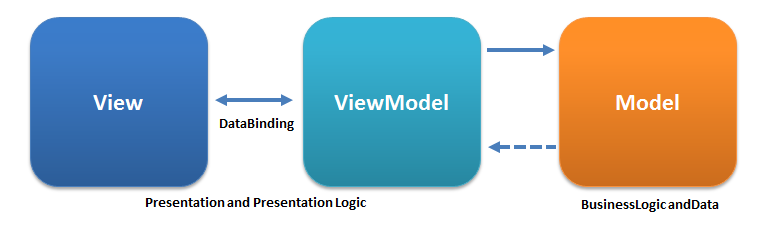
\includegraphics[scale=0.8]{../images/mvvm.png}
	\caption{Il design pattern Model View ViewModel}
\end{center}
\end{figure}
\begin {itemize}
\item\textbf{Model}: definisce l'organizzazione dei dati e ne specifica le modalità di accesso. Nel sistema Quizzipedia è situato nella parte server che opera sulla sottostante base di dati. Fa parte del Model anche la componente \emph{Parser} che opera sui dati prima che essi vengano salvati nel DBMS.
\item\textbf{View}: rappresenta l'interfaccia grafica presentata all'utilizzatore, la quale visualizza i dati e cattura le interazioni dell'utente. Nel pattern \emph{MVVM} è puramente dichiarativa, definita attraverso linguaggi di markup. 
\item\textbf{ViewModel}: è la proiezione di una parte del Model per una View; realizza il \emph{data-binding} con gli elementi della View e implementa la logica dell'applicazione. 
Realizza il disaccoppiamento totale dalla componente View dal Model.
	\end {itemize}
	Altre possibili architetture sono state prese in considerazione, ma i framework scelti, pensati per la creazione di applicazioni single-page reattive, hanno indirizzato la scelta verso il pattern \emph{MVVM}, che si adatta particolarmente all'utilizzo di AngularJS e al sistema di comunicazione client-server implementato da Meteor (publish-subscribe).

	\subsection{Descrizione del componente Model}
	Il Model, situato nella parte server del sistema svolge le seguenti funzioni:
	\begin{itemize}
		\item Interagisce con un database MongoDB nel quale vengono salvati i dati del sistema (ad es. domande, quiz, statistiche, utenti). Fornisce quindi adeguate funzionalità di salvataggio e caricamento da database di tali dati.
		\item Al momento del salvataggio di una nuova domanda esegue il \emph{parsing} del codice QML tramite un componente chiamato \emph{Parser}. Se la domanda è sintatticamente corretta può essere salvata nel database.
		\item Offre un'interfaccia logica di accesso al ViewModel attraverso la quale richiedere dati e operazioni su di essi, tramite funzionalità del framework Meteor come il \emph{Publishing} e i \emph{Methods}.
	\end{itemize}
	\subsection{Descrizione del componente View}
	La componente View rappresenta l'interfaccia grafica che visualizza i dati del ViewModel e offre le funzionalità del sistema all'utente; la View si occupa quindi solamente della rappresentazione grafica dei dati e non ha alcun contatto diretto con essi. Essendo un'interfaccia web verrà realizzata tramite HTML5 e CSS3 per le parti statiche e con l'utilizzo di template AngularJS per le parti dinamiche. Per assicurare uno stile coerente tra le pagine web e migliorare l'adattabilità a piattaforme mobile verrà utilizzato il framework CSS \emph{Materialize}.
	\subsection{Descrizione del componente ViewModel}
	Il ViewModel ricopre tre ruoli fondamentali: realizza il \emph{data-binding} con i componenti della View, cattura ed elabora gli input degli utenti e s'interfaccia col Model per richiedere e inviare dati. Per svolgere le proprie funzioni possiede le seguenti caratteristiche:
	\begin{itemize}
		\item Conosce i riferimenti alle altre due componenti. Il ViewModel è l'unica componente che conosce entrambe le altre e facendo da singolo tramite tra Model e View permette il loro totale disaccoppiamento;
		\item E' in grado di elaborare gli input della View e tradurli in azioni sul Model e sulla View stessa tramite il meccanismo del \emph{data-binding}.  
		\item E' responsabile della traduzione delle domande dal formato QML a formato HTML visualizzabile da browser, tramite un componente \emph{Interpreter}.  Tale funzionalità viene richiesta ogni qualvolta il ViewModel richiede e riceve dal Model una domanda in formato QML.
		\item Richiede dati al Model tramite la tecnica \emph{publish-subscribe} di Meteor.
		\item Gestisce la somministrazione di un questionario ad un utente, domanda dopo domanda, fino alla consegna e valutazione.
	\end{itemize}
	\newpage	
	\section{Tecnologie e strumenti utilizzati}
	\subsection{HTML5}
	Linguaggio di markup per la progettazione di pagine Web. Richiesto espressamente nel capitolato per la creazione dell'interfaccia utente (mi pare, devo controllare).
	\begin{itemize}
		\item\textbf{Utilizzo}: viene utilizzato per creare la GUI che permette all'utente di accedere al sistema mediante browser.
		\item\textbf{Vantaggi}: favorisce la portabilità su diversi dispositivi (desktop, smartphone, tablet...) e browser.
Sono punti a favore anche l'elevata compatibilità con tecnologie quali CSS3 e Javascript.
		\item\textbf{Svantaggi}: essendo HTML5 un linguaggio non ancora standard il rischio nel suo utilizzo è l'instabilità dei tag utilizzati. Un tag oggi accettato potrebbe essere modificato in un futuro prossimo, rendendo la visualizzazione dell'interfaccia utente dipendente dal stabilità dei tag utilizzati. 
	\end{itemize}
	\subsection{CSS3}
	Principale linguaggio usato per la formattazione di pagine HTML.
	\begin{itemize}
		\item\textbf{Utilizzo}: Viene utilizzato per formattare il codice HTML,
ovvero creare fogli di stile che permettono allo sviluppatore di modificare alcuni aspetti grafici della pagina Web.
		\item\textbf{Vantaggi}: Richiede un minor sforzo di interpretazione da parte del browser ed è leggero da scaricare.
		\item\textbf{Svantaggi}: Può presentare problemi di compatibilità con browser meno recenti.
	\end{itemize}
	\subsection{Materialize}
	Materialize è un framework CSS basato sull'idea di design "Material Design" di Google.
	\begin{itemize}
		\item\textbf{Utilizzo}: verrà utilizzato per la formattazione delle pagine web.
		\item\textbf{Vantaggi}: un tale framework aiuta l'applicazione a mantenere uno stile coerente in tutte le sue parti, e mette a disposizione una vasta scelta ci classi CSS preconfezionate, esonerando lo sviluppatore dalla necessita di definirne di proprie. Aumenta inoltra l'adattabilità (responsiveness) delle pagine HTML a diversi supporti (desktop, mobile, etc.).
		\item\textbf{Svantaggi}: necessità di un breve tempo di studio per impararne le classi e il corretto utilizzo.
	\end{itemize}
	\subsection{Javascript}
	E' un linguaggio di scripting debolmente orientato agli oggetti, utilizzato nelle applicazioni
Web. Viene interpretato all'interno del browser. Permette di definire funzionalità simili a
quelle offerte da C++ e Java, quali cicli e strutture di controllo.
Viene solitamente affiancato a pagine statiche HTML per poter gestire i contenuti dinamicamente, offrendo funzionalità che il linguaggio di markup non può offrire.
	\begin{itemize}
		\item\textbf{Utilizzo}: nel sistema Quizzipedia Javascript sarà ampiamente utilizzato. La quasi totalità delle componenti della ViewModel sarà realizzata in Javascript, per gestire la parte logica dell'applicazione gli elementi dinamici dell'interfaccia.
		\item\textbf{Vantaggi}: eseguito lato Client (sul browser) non sovraccarica il Server per l'esecuzione di richieste complesse. Permette un maggior livello d'interattività dell'interfaccia utente.
		\item\textbf{Svantaggi}: per script sorgenti molto corposi, può risultare oneroso in termini di
tempo lo scaricamento dei contenuti. Deve, inoltre, fare affidamento ad un linguaggio
che possa fisicamente effettuare transazioni di dati quando lo script esegue operazioni
su oggetti remoti (eg: database).
E' altresì un linguaggio non tipizzato, quindi occorre porre attenzione ai tipi delle
variabili che non sono dichiarati, ma variano dinamicamente.
		\item\textbf{Variabili e oggetti}: le variabili se sono dichiarate all'interno di una funzione sono
visibili solo all'interno di essa; se sono invece esterne sono globali. Vengono dichiarate
con la keyword \emph{var} o semplicemente assegnando loro un valore.
Ogni elemento in JavaScript è un tipo primitivo o un oggetto.
Gli oggetti sono entità dotate di unicità (sono uguali solo a sé stessi) e identificabili
con vettori associativi, che associano nomi di proprietà a valori.
	\end{itemize}
	\subsection{Node.js}
	 Node.js è un framework event-driven per il motore JavaScript V8, relativo all'utilizzo server-side di Javascript.
	\begin{itemize}
		\item\textbf{Utilizzo}: Tecnologia imposta dal proponente per la gestione della base di dati, e in generale della parte server, su cui poggia il sistema Quizzipedia.
		\item\textbf{Vantaggi}: Node.js offre prestazioni eccellenti per lo scripting server-side e una velocità superiore rispetto alla concorrenza. Il modello event-driven su cui si basa si adatta inoltre molto bene agli scopi del progetto. Secondariamente, questa tecnologia cross-platform ha suscitato molto di più l'interesse del team che se ne intende avvalere rispetto a Tomcat, l'altra tecnologia proposta dal proponente.
		\item\textbf{Svantaggi}: Il design del linguaggio impedisce alcune ottimizzazioni delle operazioni e la gestione dei tipi non è confortevole come in altri concorrenti.
	\end{itemize}
	\subsection{MongoDB}
	MongoDB è un DBMS non relazionale, orientato ai documenti. Classificato come un database di tipo NoSQL, MongoDB si allontana dalla struttura tradizionale basata su tabelle dei database relazionali in favore di documenti in stile JSON con schema dinamico rendendo l'integrazione di dati di alcuni tipi di applicazioni più facile e veloce.
	\begin{itemize}
		\item\textbf{Utilizzo}: Base di dati con lo scopo di memorizzare domande e altri dati necessari al funzionamento del sistema.
		\item\textbf{Vantaggi}: I dati non sono ristretti da alcun tipo di schema, il sistema è facilmente scalabile in caso di necessità, il livello di consistenza dei dati può essere definito a piacere, tecnologia open-source semplice da padroneggiare, in particolare il gruppo è già familiare con la sintassi JSON usata da MongoDB per la memorizzazione delle informazioni.
		\item\textbf{Svantaggi}: Minore flessibilità per quanto riguarda la formulazione delle query e elevata dimensione dei dati su server rispetto a tecnologie più tradizionali.
	\end{itemize}
	\subsection{AngularJS}
	AngularJS è un framework strutturale per la costruzione di applicazioni web. Permette di estendere la sintassi HTML con componenti della propria applicazione mantenendo comunque una stretta separazione tra i dati e la loro rappresentazione rispettando il pattern MVC.
	\begin{itemize}
		\item\textbf{Utilizzo}: Verrà utilizzato come renderer dei template della user interface di cui si occupa Meteor.
		\item\textbf{Vantaggi}: Fornisce la possibilità di creare Single Page Application in modo pulito e mantenibile facendo utilizzo di dependency injection e rispettando il principio di separazione degli interessi. Le componenti costruite con AngularJS sono facilmente riusabili e testabili. Elevata compatibilità con diversi tipi di browser.
		\item\textbf{Svantaggi}: A livello di codifica, i concetti di scope inheritance e dynamic scoping possono spesso sovrapporsi producendo del codice che non si comporta sempre allo stesso modo a run time e complicandone di conseguenza la verifica. 
		Il framework Meteor permette l'utilizzo di AngularJS come libreria di rendering, tuttavia Meteor ha un proprio linguaggio di templating (Blaze) meglio integrato nel framework (svantaggio ripagato dalla popolarità di AgularJS). 
		Essendo un framework scritto interamente in Javascript in caso l'utente disabiliti Javascript tutto il funzionamento dell'applicazione verrebbe compromesso.
		La scarsa conoscenza del framework da parte del gruppo impone di preventivare alcune ore di tempo per impararne le funzionalità.
	\end{itemize}
	\subsection{Meteor}
	Meteor è una piattaforma full-stack Javascript per la costruzione di mobile e web apps. Semplifica la creazione di applicazioni real time offrendo un ecosistema completo atto al loro sviluppo e alla loro fruizione.
	\begin{itemize}
		\item\textbf{Utilizzo}: Questa tecnologia contribuirà alla realizzazione del cuore principale dell'applicazione Quizzipedia.
		\item\textbf{Vantaggi}: Framework abbastanza semplice da imparare ad utilizzare, ideale per lo sviluppo di applicazioni web real time, sia front-end che back-end vengono codificati principalmente usando solo Javascript, presenza di package che semplificano e velocizzano lo sviluppo dell'applicazione, alta scalabilità del progetto.
		\item\textbf{Svantaggi}: Il modo in cui alcuni componenti core della tecnologia si interfacciano potrebbe limitare la libertà degli sviluppatori. Esperienze precedenti con la tecnologia scarse o nulle dei componenti del Team 404, tempi abbastanza considerevoli dovranno essere impiegati nel conseguimento di una buona padronanza del framework.
	\end{itemize}
	\newpage
	\section{Risorse necessarie}
	Dato che il progetto sarà sviluppato con le tecnologie di cui sopra, per lo sviluppo il gruppo avrà bisogno di risorse quali:
	\begin{itemize}
	\item un server integrato in un hosting Web che supporti un database MongoDB, scripting Node.js e il deployment di un'applicazione basata su Meteor. E' stato scelto il servizio di hosting OpenShift.
	\item un buon IDE per lo sviluppo web che faciliti la creazione di codice HTML, CSS e Javascript (ad es. NetBeans, Eclipse, Aptana Studio).
	\item un editor UML per la creazione dei diagrammi UML  di questo documento e della Definizione di Prodotto. Sono stati usati Astah e StarUML.
	\item scaricare e installare il framework Meteor per consentire lo sviluppo e il testing dell'applicazione in locale.
	\end{itemize}
	\newpage
	
	\section{Diagrammi dei packages}
		\subsection{Server}
		Nella parte \emph{Server} del sistema lavorano gli elementi del Model.
			\subsubsection{Package della componente Model}
	\begin{figure}[h!]
	\begin{center}
		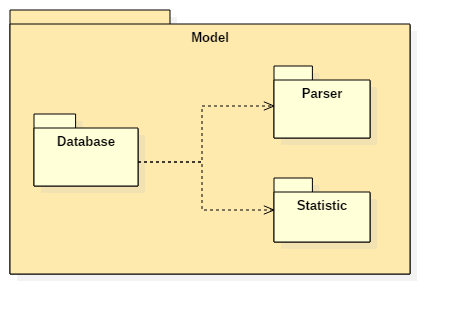
\includegraphics[scale=0.65]{../images/ModelPackage.png}
		\caption{Package della componente Model}
	\end{center}
	\end{figure}
	Il package per il componente Model del pattern architetturale MVP contiene i seguenti sotto packages:
	\begin{itemize}
		\item\textbf{Database:} questo package si occuperà di gestire le richieste in arrivo dal Presenter e avviserà quest'ultimo ogni qualvolta si verifica un cambiamento dei dati salvati nel sistema tramite appositi eventi; Per fare ciò si avvale delle classi:
			\begin{itemize}
				\item\textit{UserManager}
				\item\textit{QuizManager}
				\item\textit{QuestionManager}
			\end{itemize}
		\item\textbf{Parser:} questo package fornisce funzionalità per il controllo sintattico rispetto a QML; Per fare ciò si avvale delle classi:
			\begin{itemize}
				\item\textit{Parser}
			\end{itemize}
		\item\textbf{Statistic:} questo package fornisce classi per il raccoglimento delle statistiche relative ai quesiti, questionari ed utenti; Per fare ciò si avvale delle classi:
			\begin{itemize}
				\item\textit{Statistics}
			\end{itemize}
			\item\textbf{Publishers:} questo package fornisce classi per la pubblicazione delle collezioni presenti sul database:
			\begin{itemize}
				\item\textit{UserPublisher}
				\item\textit{QuizPublisher}
				\item\textit{QuestionPublisher}
			\end{itemize}
		\end{itemize}
		\newpage
		\subsection{Client}
		Nella parte \emph{Client} del sistema risiedono i componenti dalla View e del ViewModel.
			\subsubsection{Package della componente View}
	\begin{figure}[h!]
	\begin{center}
		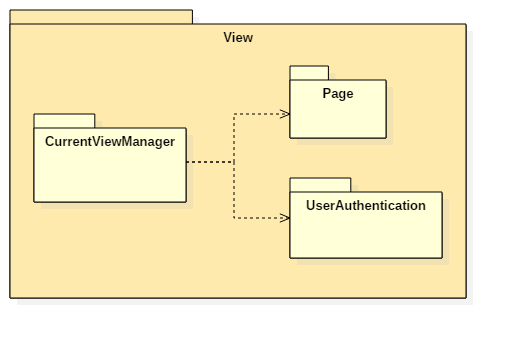
\includegraphics[scale=0.6]{../images/ViewPackage.png}
		\caption{Package della componente View}
	\end{center}
	\end{figure}
	Il package per il componente View del pattern architetturale MVVM contiene i seguenti sotto packages:
	\begin{itemize}
		\item\textbf{Pages:} contiene la classe astratta \textit{Page}, che rappresenta una generica pagina del sistema, più tutte le sue derivazioni concrete, una per ogni pagina prevista. Le pagine possono utilizzare al loro interno dei template per visualizzare situazioni standard gestite da una componente nel package Templates.
		\item\textbf{Templates:} contiene le classi che rappresentano le componenti utilizzabili dalle pagine per visualizzare situazioni o modelli di dati simili tra loro. Si ha così un disaccoppiamento di quali elementi una pagina contiene da come questi sono realizzati.\\
\\
\end{itemize}	
\newpage
			\subsubsection{Package della componente ViewModel}
	\begin{center}
		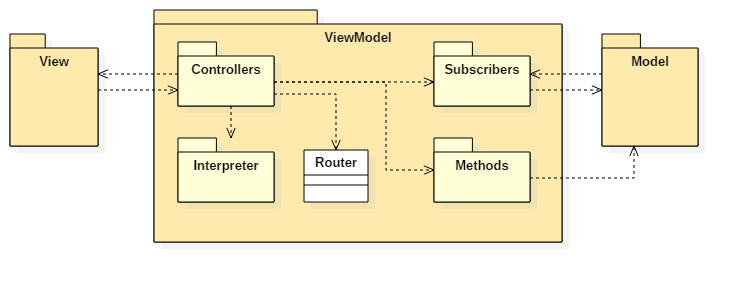
\includegraphics[scale=0.6]{../images/ViewModelPackage.png}
	\end{center}
	Gli elementi del package collaborano e interagiscono con l'obiettivo comune di realizzare il data-binding con i componenti della View e interagire col Model per richiedere e aggiornare i dati. \\
	Il package del ViewModel contiene i seguenti sub-packages:
	\begin{itemize}
	\item \textbf{Controllers}:
	Il package contiene al suo interno le classi:
	\begin{itemize}
		\item \textit{NewQuestionController}
		\item \textit{NewQuizController}
		\item \textit{QuizManagementController}
		\item \textit{QuizListController}
		\item \textit{QuizDetailsController}
		\item \textit{DeleteQuestionController}
		\item \textit{DeleteQuizController}
		\item \textit{QuestionsManagementController}
		\item \textit{QMLEditorController}
		\item \textit{}
		\item \textit{}
		\item \textit{}
		\item \textit{}
		\item \textit{}
		\item \textit{}
		\item \textit{}
	\end{itemize}	
	\item \textbf{Subscribers}:
	Il package contiene al suo interno le classi:
	\begin{itemize}
		\item \textit{}
		\item \textit{}
	\end{itemize}
	
	\item \textbf{QuestionManager}:
	Il package \emph{QuestionManager} espone le funzionalità necessarie alla creazione e gestione di domande. Per permettere al package di essere estendibile in futuro con domande in diversi formati, le classi al suo interno sono organizzate seguendo il pattern \emph{Abstract Factory}. \\
	Il package contiene al suo interno le classi:
	\begin{itemize}
		\item \textit{QuestionFactory}
		\item \textit{Question}
		\item \textit{QML2HTMLFactory}
		\item \textit{HTMLQuestion}
		\item \textit{Translator}
	\end{itemize}
	
	\item\textbf{QuizManager}:
	Il Package \emph{QuizManager} espone le funzionalità necessarie alla creazione e gestione di quiz, collaborando con il package \emph{QuestionManager}. Per disaccoppiare la creazione di un quiz dalle domande che lo compongono, la classi all'interno del package seguono la struttura del design pattern \emph{Builder}.\\ 
	Il package contiene al suo interno le classi:
	\begin{itemize}
		\item \textit{QuizDirector}
		\item \textit{QuizBuilder}
		\item \textit{Quiz}
	\end{itemize}
	
	\item \textbf{Interpreter}:
	Il package \emph{Interpreter} è responsabile della traduzione di testo QML in codice HTML5 visualizzabile da browser. Per permettere al package di essere estendibile in futuro con nuovi tipi di "Interpreter", le classi al suo interno sono organizzate seguendo il pattern \emph{Abstract Factory} . \\
	Il package contiene al suo interno le seguenti classi:
	\begin{itemize}
	\item \textit{Interpreter}
	\item \textit{InterpreterFactory}
	\item \textit{QMLInterpreterFactory}
	\item \textit{QMLInterpreter}
	\item \textit{QML2HTMLInterpreter}
	\end{itemize}
	
	\end{itemize}
	
	\section{Diagrammi delle classi del Server}
		\subsection{Diagrammi delle classi del Model}
			\subsubsection{Package Database}
			\begin{center}
				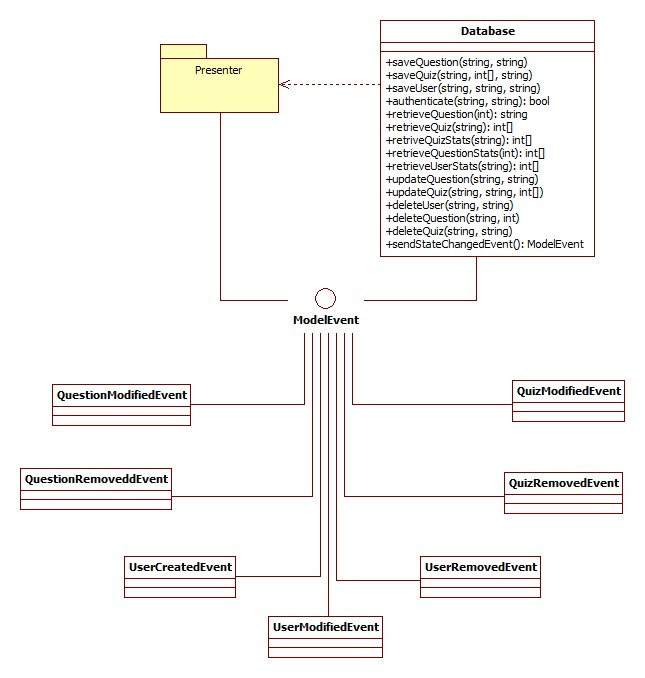
\includegraphics[scale=0.6]{../images/Database.jpg}
			\end{center}
 			\subsubsubsection{Classe Database}
 			\begin{itemize}
		    	\item\textbf{Funzione del componente:} la classe permettera' l'inserimento, la lettura, la modifica e la rimozione dei dati all'interno del database
			\item\textbf{Relazioni d'uso di altri componenti:} interagisce con il Presenter, inviando o ricevendo dati sulla base delle richieste di quest'ultimo
			\item\textbf{Attivita' svolte e dati trattati:} ogni metodo della classe consente l'inserimento, la lettura, la modifica e la rimozione di dati dal database, in seguito alla quale si possono verificare eventi per notificare al Presenter
			\end{itemize}
			\subsubsubsection{Interfaccia ModelEvent}
			\begin{itemize}
		    	\item\textbf{Funzione del componente:} l'interfaccia identifichera' dei particolari eventi che richiedono l'intervento del Presenter
			\item\textbf{Relazioni d'uso di altri componenti:} questa interfaccia verra implementata da classi che andranno a specificare un particolare tipo di evento
			\end{itemize}
			\subsubsubsection{Classe QuestionModifiedEvent}
			\begin{itemize}
		    	\item\textbf{Funzione del componente:} la classe specifica la modifica di un quesito nel database
				\item\textbf{Relazioni d'uso di altri componenti:} implementa l'interfaccia ModelEvent
				\item\textbf{Attivita' svolte e dati trattati:} segnala al Presenter il verificarsi della modifica di un quesito
			\end{itemize}
			\subsubsubsection{Classe QuestionRemovedEvent}
			\begin{itemize}
		    	\item\textbf{Funzione del componente:} la classe specifica la rimozione di un quesito nel database
				\item\textbf{Relazioni d'uso di altri componenti:} implementa l'interfaccia ModelEvent
				\item\textbf{Attivita' svolte e dati trattati:} segnala al Presenter il verificarsi della rimozione di un quesito
			\end{itemize}
			\subsubsubsection{Classe QuizModifiedEvent}
			\begin{itemize}
		    	\item\textbf{Funzione del componente:} la classe specifica la modifica di un quiz nel database
				\item\textbf{Relazioni d'uso di altri componenti:} implementa l'interfaccia ModelEvent
				\item\textbf{Attivita' svolte e dati trattati:} segnala al Presenter il verificarsi della modifica di un quiz
			\end{itemize}
			\subsubsubsection{Classe QuizRemovedEvent}
			\begin{itemize}
		    	\item\textbf{Funzione del componente:} la classe specifica la rimozione di un quiz nel database
				\item\textbf{Relazioni d'uso di altri componenti:} implementa l'interfaccia ModelEvent
				\item\textbf{Attivita' svolte e dati trattati:} segnala al Presenter il verificarsi della rimozione di un quiz
			\end{itemize}
			\subsubsubsection{Classe UserCreatedEvent}
			\begin{itemize}
		    	\item\textbf{Funzione del componente:} la classe specifica l'aggiunta di un nuovo utente nel database
				\item\textbf{Relazioni d'uso di altri componenti:} implementa l'interfaccia ModelEvent
				\item\textbf{Attivita' svolte e dati trattati:} segnala al Presenter il verificarsi dell'aggiunta di un nuovo utente
			\end{itemize}
			\subsubsubsection{Classe UserModifiedEvent}
			\begin{itemize}
		    	\item\textbf{Funzione del componente:} la classe specifica la modifica di un utente nel database
				\item\textbf{Relazioni d'uso di altri componenti:} implementa l'interfaccia ModelEvent
				\item\textbf{Attivita' svolte e dati trattati:} segnala al Presenter il verificarsi della modifica di un utente
			\end{itemize}
			\subsubsubsection{Classe UserRemovedEvent}
			\begin{itemize}
		    	\item\textbf{Funzione del componente:} la classe specifica la rimozione di un utente nel database
				\item\textbf{Relazioni d'uso di altri componenti:} implementa l'interfaccia ModelEvent
				\item\textbf{Attivita' svolte e dati trattati:} segnala al Presenter il verificarsi della rimozione di un utente
			\end{itemize}
			
			\subsubsection{Package Parser}
			\begin{center}
				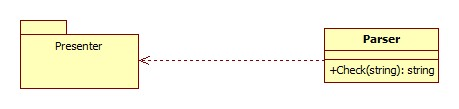
\includegraphics[scale=0.6]{../images/Parser.jpg}
			\end{center}
 			\subsubsubsection{Classe Parser}
 			\begin{itemize}
		    	\item\textbf{Funzione del componente:} controlla che il testo fornito risulti corretto secondo la sintassi QML
			\item\textbf{Attivita' svolte e dati trattati:} il Parser controlla che il testo fornito in input rispetta la sintassi QML e fornisce in caso di errore un messaggio avvertendo l'utente di dove si trova l'errore e la tipologia
			\end{itemize}
			
			\subsubsection{Package Statistiche}
			\begin{center}
				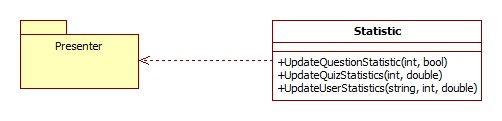
\includegraphics[scale=0.6]{../images/Statistics.jpg}
			\end{center}
 			\subsubsubsection{Classe Statistic}
 			\begin{itemize}
		    	\item\textbf{Funzione del componente:} questa classe fornisce funzionalita' per il raccoglimento delle statistiche all'interno di Quizzipedia
			\item\textbf{Attivita' svolte e dati trattati:} la classe aggiornera' le statistiche relative ai quesiti, questionari ed utenti.
			Per i quesiti verranno indicati il numero di volte che e' stato proposto e il numero di risposte corrette.
			Per i questionari verranno indicati le valutazioni medie ottenute dagli utenti e il numero di volte che e' stato proposto.
			Per gli utenti verranno indicati la valutazione migliore e la media dei tentativi eseguiti su singolo quiz
			\end{itemize}
	\section{Diagrammi delle classi del Client}
		\subsection{Diagrammi delle classi della View}	
		
	\subsubsection{Package Pages}
		\begin{center}
			\centerline{\includegraphics[scale=0.6]{"../../images/Pages".png}}
		\end{center}
		\subsubsubsection{Interfaccia Page}
			\begin{itemize}
		    		\item\textbf{Funzione del componente:} rappresenta una pagina web
				\item\textbf{Relazioni d'uso di altri componenti:} interfaccia che viene concretizzata dalle sue classi derivate che rappresenta una pagina dell'applicazione
				\item\textbf{Attività svolte e dati trattati:} fornisce il contratto di una pagina deve soddisfare ovvero visualizzare il proprio contenuto. Inoltre fornisce un tipo che gli altri package possono utilizzare per riferirsi ad una qualsiasi pagina.
			\end{itemize}
		\subsubsubsection{Classe LoginPage}
			\begin{itemize}
		    		\item\textbf{Funzione del componente:} visualizza il form di autenticazione e permette il login dell'utente. Fornisce inoltre un link alla pagina di registrazione e uno alla pagina di recupero della password 
				\item\textbf{Relazioni d'uso di altri componenti:} concretizza l'interfaccia Page da cui è diretta discendente e utilizza il template LoginForm
				\item\textbf{Attività svolte e dati trattati:} permette l'autenticazione dell'utente nel sistema
			\end{itemize}
		\subsubsubsection{Classe RegistrationPage}
			\begin{itemize}
		    		\item\textbf{Funzione del componente:} visualizza il form di registrazione. Fornisce inoltre un link alla pagina di login
				\item\textbf{Relazioni d'uso di altri componenti:} concretizza l'interfaccia Page da cui è diretta discendente e utilizza il template RegistrationForm
				\item\textbf{Attività svolte e dati trattati:} permette la registrazione dell'utente nel sistema
			\end{itemize}
		\subsubsubsection{Classe PasswordRecoveryPage}
			\begin{itemize}
		  		\item\textbf{Funzione del componente:} visualizza il form per il recupero della password
				\item\textbf{Relazioni d'uso di altri componenti:} concretizza l'interfaccia Page da cui è diretta discendente e utilizza il template PasswordRecoveryForm
				\item\textbf{Attività svolte e dati trattati:} permette il recupero della password dimenticata tramite l'invio di una email
			\end{itemize}
		\subsubsubsection{Classe CategoryListPage}
			\begin{itemize}
		    		\item\textbf{Funzione del componente:} visualizza la lista delle categorie
				\item\textbf{Relazioni d'uso di altri componenti:} concretizza l'interfaccia Page da cui è diretta discendente
				\item\textbf{Attività svolte e dati trattati:} permette la selezione di una categoria che porta ad una pagina in cui vengono visualizzati tutti i questionari della categoria scelta
			\end{itemize}
		\subsubsubsection{Classe QuizListPage}
			\begin{itemize}
		    		\item\textbf{Funzione del componente:} visualizza una lista di questionari
				\item\textbf{Relazioni d'uso di altri componenti:} concretizza l'interfaccia Page da cui è diretta discendente e utilizza il template QuizList
				\item\textbf{Attività svolte e dati trattati:} permette la selezione di un questionario che porta alla pagina di compilazione del questionario scelto
			\end{itemize}
		\subsubsubsection{Classe QuizExecutionPage}
			\begin{itemize}
		    		\item\textbf{Funzione del componente:} visualizza un questionario (una domanda alla volta) e tutti i dati relativi (tempo rimasto, numero domande, ecc...)
				\item\textbf{Relazioni d'uso di altri componenti:} concretizza l'interfaccia Page da cui è diretta discendente e utilizza il template QuestionCompilation
				\item\textbf{Attività svolte e dati trattati:} permette la compilazione di un questionario
			\end{itemize}
		\subsubsubsection{Classe QuizResultsPage}
			\begin{itemize}
		    		\item\textbf{Funzione del componente:} visualizza i risultati del questionario appena compilato
				\item\textbf{Relazioni d'uso di altri componenti:} concretizza l'interfaccia Page da cui è diretta discendente e utilizza il template QuizResults
				\item\textbf{Attività svolte e dati trattati:} permette la compilazione di un questionario
			\end{itemize}
		\subsubsubsection{Classe QuestionManagmentPage}
			\begin{itemize}
		    		\item\textbf{Funzione del componente:} visualizza la lista delle domande create dall'utente
				\item\textbf{Relazioni d'uso di altri componenti:} concretizza l'interfaccia Page da cui è diretta discendente e utilizza il template QuestionList
				\item\textbf{Attività svolte e dati trattati:} permette l'accesso alle pagine di creazione di una nuova domanda e modifica di una domanda esistente. Permette inoltre l'eliminazione di una domanda
			\end{itemize}
		\subsubsubsection{Classe QuestionCreationPage}
			\begin{itemize}
		    		\item\textbf{Funzione del componente:} visualizza il form di creazione di una nuova domanda
				\item\textbf{Relazioni d'uso di altri componenti:} concretizza l'interfaccia Page da cui è diretta discendente e utilizza il template QuestionForm
				\item\textbf{Attività svolte e dati trattati:} permette la creazione di una nuova domanda
			\end{itemize}
		\subsubsubsection{Classe QuestionUpdatePage}
			\begin{itemize}
		    		\item\textbf{Funzione del componente:} visualizza il form di modifica di una domanda
				\item\textbf{Relazioni d'uso di altri componenti:} concretizza l'interfaccia Page da cui è diretta discendente e utilizza il template QuestionForm
				\item\textbf{Attività svolte e dati trattati:} permette la modifica di una domanda
			\end{itemize}
		\subsubsubsection{Classe QuizCreationPage}
			\begin{itemize}
		    		\item\textbf{Funzione del componente:} visualizza il form di creazione di un nuovo questionario
				\item\textbf{Relazioni d'uso di altri componenti:} concretizza l'interfaccia Page da cui è diretta discendente e utilizza il template QuizCreationForm
				\item\textbf{Attività svolte e dati trattati:} permette la creazione di un nuovo questionario
			\end{itemize}
			
	\subsubsection{Package Templates}
		\begin{center}
			\includegraphics[scale=0.6]{"../../images/Templates".png}
		\end{center}
		\subsubsubsection{Classe QuestionList}
			\begin{itemize}
				\item\textbf{Funzione del componente:} visualizza una lista di domande
				\item\textbf{Relazioni d'uso di altri componenti:} composta da Question
			\end{itemize}
		\subsubsubsection{Classe Question}
			\begin{itemize}
				\item\textbf{Funzione del componente:} visualizza una domanda inserita in una lista
				\item\textbf{Relazioni d'uso di altri componenti:} usata solo da QuestionList per creare la lista
			\end{itemize}
		\subsubsubsection{Classe QuizList}
			\begin{itemize}
				\item\textbf{Funzione del componente:} visualizza una lista di quiz
				\item\textbf{Relazioni d'uso di altri componenti:} composta da Quiz
			\end{itemize}
		\subsubsubsection{Classe Quiz}
			\begin{itemize}
				\item\textbf{Funzione del componente:} visualizza un quiz inserito in una lista
				\item\textbf{Relazioni d'uso di altri componenti:} usata solo da QuizList per creare la lista
			\end{itemize}
		\subsubsubsection{Classe QuestionCompilation}
			\begin{itemize}
				\item\textbf{Funzione del componente:} visualizza una domanda e ne permette la compilazione
			\end{itemize}
		\subsubsubsection{Classe QuestionForm}
			\begin{itemize}
				\item\textbf{Funzione del componente:} visualizza il form per i dati di una domanda. Utilizzabile sia per la creazione che per la modifica della domanda (se viene modificata una domanda già esistente nei campi vengono inseriti i valori attuali)
			\end{itemize}
		\subsubsubsection{Classe QuizCreation}
			\begin{itemize}
				\item\textbf{Funzione del componente:} visualizza il form di creazione di un questionario
			\end{itemize}
		\subsubsubsection{Classe QuizResults}
			\begin{itemize}
				\item\textbf{Funzione del componente:} visualizza i risultati ottenuti in seguito alla compilazione di un quiz
			\end{itemize}
		\subsubsubsection{Classe SearchForm}
			\begin{itemize}
				\item\textbf{Funzione del componente:} visualizza un form per l'inserimento dei dati desiderati e l'avvio della ricerca
			\end{itemize}
		\subsubsubsection{Classe RegistrationForm}
			\begin{itemize}
				\item\textbf{Funzione del componente:} visualizza un form per la registrazione di un nuovo utente
			\end{itemize}
		\subsubsubsection{Classe LoginForm}
			\begin{itemize}
				\item\textbf{Funzione del componente:} visualizza un form per l'autenticazione di un utente
			\end{itemize}
		\subsubsubsection{Classe PasswordRecoveryForm}
			\begin{itemize}
				\item\textbf{Funzione del componente:} visualizza un form per il recupero della password dimenticata
			\end{itemize}
			
			\newpage
		\subsection{Diagrammi delle classi del ViewModel}
\subsubsection{Package Controllers}
\begin{figure}[h!]
	\begin{center}
		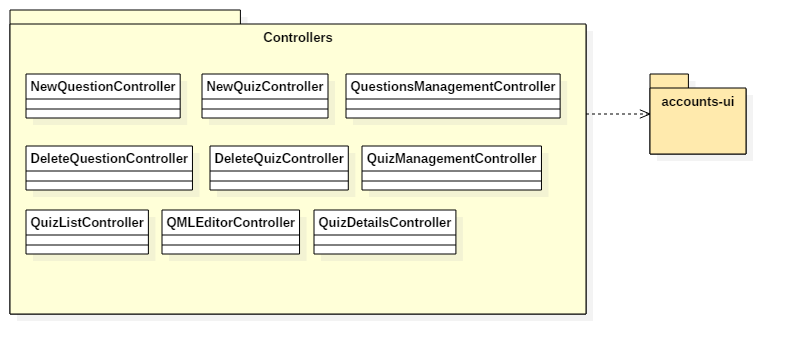
\includegraphics[scale=0.6]{../images/ControllersClass.png}
		\caption{Diagramma delle classi del package Controllers}
	\end{center}
\end{figure}

\subsubsubsection{Classe NewQuestionController}

\begin{itemize}
	\item\textbf{Funzione del componente}: la classe permette di gestire la creazione di una nuova domanda;
	\item\textbf{Relazione d'uso di altre componenti}: il controller è collegato al template. Si relaziona inoltre con  l'editor QML;
	\item\textbf{Attività svolte e dati trattati}: Fornisce le funzionalità per la creazione di una domanda, quali la scelta della categoria e l'inserimento del testo, e espone la funzione di salvataggio dei dati inseriti che compongono la nuova domanda.
\end{itemize}

\subsubsubsection{Classe NewQuizController}

\begin{itemize}
	\item\textbf{Funzione del componente}: la classe permette di gestire la creazione di un nuovo quiz (questionario); 
	\item\textbf{Relazione d'uso di altre componenti}: il controller è collegato al template;
	\item\textbf{Attività svolte e dati trattati}: fornisce le funzionalità per la creazione del nuovo quiz, tramite la scelta di più domande e la scelta della categoria. Espone la funzione di salvataggio del nuovo quiz.
\end{itemize}

\subsubsubsection{Classe QuizListController}

\begin{itemize}
	\item\textbf{Funzione del componente}:  la classe permette il caricamento e la visualizzazione della lista di quiz disponibili nel sistema;
	\item\textbf{Relazione d'uso di altre componenti}: il controller è collegato al templat.; Si relaziona inoltre con il modulo QuizDetails per la visualizzazione dei dettagli di un quiz;
	\item\textbf{Attività svolte e dati trattati}: la classe si occupa di caricare la lista aggiornata dei quiz creati dagli utenti, e fornisce funzionalità di ordinamento della stessa e di selezione dei singoli quiz per la visualizzazione dei dettagli. 
\end{itemize}

\subsubsubsection{Classe QuizDetailsController}

\begin{itemize}
	\item\textbf{Funzione del componente}: la classe permette di visualizzare le informazioni generali di un quiz, una volta selezionato dalla lista dei quiz;
	\item\textbf{Relazione d'uso di altre componenti}: il controller è collegato al template. Si relaziona inoltre con il modulo QuizList.
	\item\textbf{Attività svolte e dati trattati}: la classe si occupa di recuperare e rendere visualizzabili le informazioni relative ad un singolo quiz.
\end{itemize}

\subsubsubsection{Classe DeleteQuestionController}

\begin{itemize}
	\item\textbf{Funzione del componente}: la classe fornisce le funzionalità necessarie alla cancellazione di una domanda precedentemente creata;
	\item\textbf{Relazione d'uso di altre componenti}: il controller è collegato al template. Si relaziona inoltre con il package Methods.
	\item\textbf{Attività svolte e dati trattati}: la classe si occupa di richiedere la cancellazione di una domanda, precedentemente creata dall'utente, dal sistema.
\end{itemize}

\subsubsubsection{Classe DeleteQuizController}

\begin{itemize}
	\item\textbf{Funzione del componente}: la classe fornisce le funzionalità necessarie alla cancellazione di un quiz precedentemente creato;
	\item\textbf{Relazione d'uso di altre componenti}: il controller è collegato al template. Si relaziona inoltre con il package Methods.
	\item\textbf{Attività svolte e dati trattati}:  la classe si occupa di richiedere la cancellazione di un quiz, precedentemente creato dall'utente, dal sistema.
\end{itemize}

\subsubsubsection{Classe QuizManagementController}

\begin{itemize}
	\item\textbf{Funzione del componente}: la classe permette di gestire la somministrazione di un questionario;
	\item\textbf{Relazione d'uso di altre componenti}: il controller è collegato al template. Si relaziona inoltre con il modulo QuestionsManagement;
	\item\textbf{Attività svolte e dati trattati}: la classe si occupa di gestire la risoluzione di un questionario da parte di un utente fornendo la possibilità di navigare tra le domande, salvando le risposte dell'utente e gestendo il tempo limite. Espone la funzione di consegna del quiz compilato.
\end{itemize}

\subsubsubsection{Classe QuestionsManagementController}

\begin{itemize}
	\item\textbf{Funzione del componente}: la classe permette di gestire la somministrazione di una singola domanda all'interno di un questionario;
	\item\textbf{Relazione d'uso di altre componenti}: il controller è collegato al template. Si relaziona inoltre con il modulo QuizManagement;
	\item\textbf{Attività svolte e dati trattati}: la classe si occupa di recuperare i dati associati ad una singola domanda di un questionario e di presentarli all'utente. Tali operazioni si svolgono durante la somministrazione all'utente di un questionario.
\end{itemize}

\subsubsubsection{Classe QMLEditorController}

\begin{itemize}
	\item\textbf{Funzione del componente}: fornisce le funzionalità per creare e modificare una domanda tramite editor QML;
	\item\textbf{Relazione d'uso di altre componenti}: il controller è collegato al template. Si relaziona inoltre con il modulo NewQuestion;
	\item\textbf{Attività svolte e dati trattati}: la classe definisce la logica dello strumento principale di creazione delle domande, l'editor QML, gestisce il testo che viene inserito e espone la funzionalità di checking sintattico del testo inserito.
\end{itemize}

\subsubsubsection{Classe Controller}

\begin{itemize}
	\item\textbf{Funzione del componente}: 
	\item\textbf{Relazione d'uso di altre componenti}: 
	\item\textbf{Attività svolte e dati trattati}:
\end{itemize}

\subsubsection{Package Subscribers}
\begin{figure}[h!]
\begin{center}
	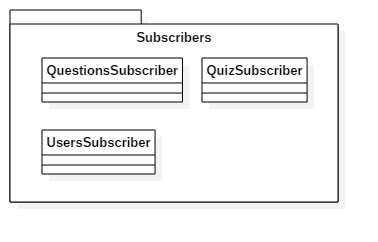
\includegraphics[scale=0.65]{../images/SubscribersClass.png}
	\caption{Diagramma delle classi del package Subscribers}
\end{center}
\end{figure}

\subsubsubsection{Classe QuestionsSubscriber}

\begin{itemize}
	\item\textbf{Funzione del componente}: la classe è necessaria ad effettuare il \emph{subscribe} relativo alla collezione di domande del sistema;
	\item\textbf{Relazione d'uso di altre componenti}: si relazione con la componente QuestionsManagementController;
	\item\textbf{Attività svolte e dati trattati}: la classe espone le funzionalità necessarie ad effettuare il subscribing di una componente del client alla collezione di domande del sistema, se questa è stata precedentemente pubblicata dal server.
\end{itemize}

\subsubsubsection{Classe QuizSubscriber}

\begin{itemize}
	\item\textbf{Funzione del componente}: la classe è necessaria ad effettuare il \emph{subscribe} relativo alla collezione di quiz del sistema;
	\item\textbf{Relazione d'uso di altre componenti}: si relazione con le componenti QuizListController e QuizManagementController;
	\item\textbf{Attività svolte e dati trattati}: la classe espone le funzionalità necessarie ad effettuare il subscribing di una componente del client alla collezione di quiz del sistema, se questa è stata precedentemente pubblicata dal server.
\end{itemize}

\subsubsubsection{Classe UsersSubscriber}

\begin{itemize}
	\item\textbf{Funzione del componente}: la classe è necessaria ad effettuare il \emph{subscribe} relativo alla collezione di utenti del sistema;
	\item\textbf{Relazione d'uso di altre componenti}: si relaziona con il package esterno 'accounts-ui';
	\item\textbf{Attività svolte e dati trattati}: la classe espone le funzionalità necessarie ad effettuare il subscribing di una componente del client alla collezione di utenti del sistema, se questa è stata precedentemente pubblicata dal server.
\end{itemize}

\subsubsection{Package Methods}
\begin{figure}[h!]
\begin{center}
	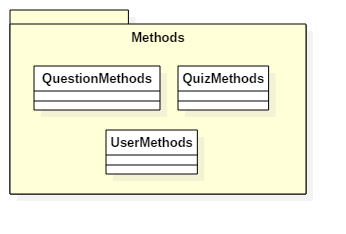
\includegraphics[scale=0.65]{../images/MethodsClass.png}
	\caption{Diagramma delle classi del package Methods}
\end{center}
\end{figure}

\subsubsubsection{Classe QuestionMethods}
\begin{itemize}
	\item\textbf{Funzione del componente}: permette al client di richiedere la modifica della collezione di domande del server;
	\item\textbf{Relazione d'uso di altre componenti}: si relaziona con le classi NewQuestionController e DeleteQuestionController;
	\item\textbf{Attività svolte e dati trattati}: espone le funzionalità di salvataggio e cancellazione di domande dal sistema.
\end{itemize}

\subsubsubsection{Classe QuizMethods}
\begin{itemize}
	\item\textbf{Funzione del componente}: permette al client di richiedere la modifica della collezione di quiz del server;
	\item\textbf{Relazione d'uso di altre componenti}: si relaziona con le classi NewQuizController e DeleteQuizController;
	\item\textbf{Attività svolte e dati trattati}: espone le funzionalità di salvataggio e cancellazione di quiz dal sistema.
\end{itemize}

\subsubsubsection{Classe UserMethods}
\begin{itemize}
	\item\textbf{Funzione del componente}: permette al client di richiedere la modifica della collezione di utenti del server;
	\item\textbf{Relazione d'uso di altre componenti}:  si relaziona con il package esterno 'accounts-ui';
	\item\textbf{Attività svolte e dati trattati}: espone le funzionalità di salvataggio e cancellazione di utenti dal sistema.
\end{itemize}
\newpage			

\subsubsection{Package Interpreter}
\begin{figure}[h!]
\begin{center}
	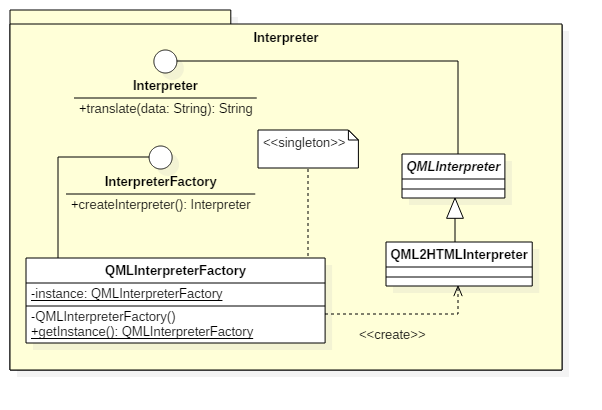
\includegraphics[scale=0.65]{../images/InterpreterClass.png}
	\caption{Diagramma delle classi del package Interpreter}
\end{center}
\end{figure}
\subsubsubsection{Interfaccia Interpreter}
\begin{itemize}
	\item\textbf{Funzione del componente}: interfaccia di base del tipo Interpreter.
	\item\textbf{Relazione d'uso di altre componenti}: può essere concretizzata in diversi tipi di Interpreter.
	\item\textbf{Attività svolte e dati trattati}: definisce il contratto degli Interpreter, cioè le operazioni di traduzione che saranno definite in ogni concretizzazione.
\end{itemize}
\subsubsubsection{Interfaccia InterpreterFactory}
\begin{itemize}
	\item\textbf{Funzione del componente}: interfaccia di base delle Factory di tipi Interpreter.
	\item\textbf{Relazione d'uso di altre componenti}: può essere concretizzata in diversi tipi di InterpreterFactory.
	\item\textbf{Attività svolte e dati trattati}: definisce il contratto delle factory, cioè le operazioni di costruzione di Interpreter che saranno definite in ogni concretizzazione.
\end{itemize}
\subsubsubsection{Classe QMLInterpreterFactory}
La classe QMLInterpreterFactory è un \emph{singleton}.
\begin{itemize}
	\item\textbf{Funzione del componente}: crea oggetti di tipo QMLInterpreter.
	\item\textbf{Relazione d'uso di altre componenti}: è concretizzazione della classe InterpreterFactory. Crea oggetti QMLInterpreter.
	\item\textbf{Attività svolte e dati trattati}: crea su richiesta oggetti di tipo QMLInterpreter.
\end{itemize}
\subsubsubsection{Classe QMLInterpreter}
\begin{itemize}
	\item\textbf{Funzione del componente}: classe astratta che rappresenta gli Interpreter che traducono codice QML in un altro formato.
	\item\textbf{Relazione d'uso di altre componenti}: è sottotipo di Interpreter. Può essere concretizzata in più tipi di QMLInterpreter.
	\item\textbf{Attività svolte e dati trattati}: definisce il contratto dei QMLInterpreter, cioè le operazioni di traduzione da QML verso altri linguaggi.
\end{itemize}
\subsubsubsection{Classe QML2HTMLInterpreter}	
\begin{itemize}
	\item\textbf{Funzione del componente}: traduce codice QML in codice HTML.
	\item\textbf{Relazione d'uso di altre componenti}: è concretizzazione di QMLInterpreter.
	\item\textbf{Attività svolte e dati trattati}: riceve in input domande in QML e le traduce in codice HTML visualizzabile da browser.
\end{itemize}
\newpage
	
	\section{Diagrammi di attività}
		\input{sezioni/attività.tex}
	\section{Diagrammi di sequenza}
		\subsection{Salvataggio di una Domanda}
	\begin{figure}[h!]
	\begin{center}
		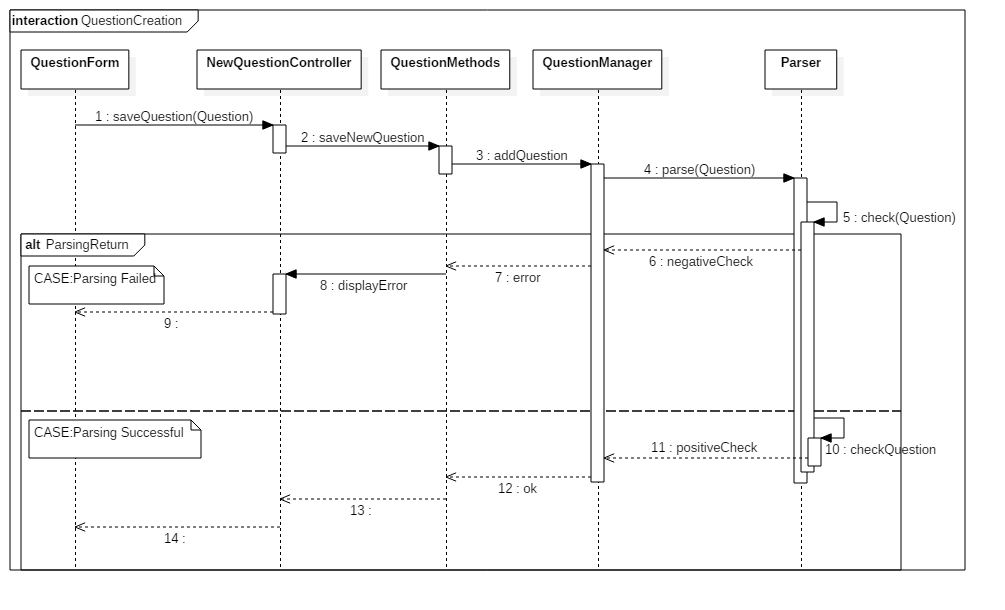
\includegraphics[scale=0.5]{../images/QuestionCreation.png}
		\caption{Diagramma di sequenza del salvataggio di una domanda}
	\end{center}
	\end{figure}
	\begin{itemize}
	\item\textbf{Precondizioni:} l'utente è autenticato nel sistema Quizzipedia e accede all'area del sito dedicata alla gestione (creazione, eliminazione e modifica) dei propri singoli quesiti.\\
	\item\textbf{Postcondizioni:} l'utente ha creato con successo una nuova domanda. La nuova domanda sarà disponibile a tutti gli utenti qualora essi decidano di creare un questionario appartenente alla stessa categoria. L'utente viene reindirizzato alla pagina di gestione questionari.\\
	\item\textbf{Descrizione:} l'utente compila il form per la creazione della nuova domanda (al cui interno ricordiamo è situato un campo adibito alla stesura del codice QML) e sottomette i dati al sistema. L'evento viene notificato alla ViewModel che chiama il Parser situato nel Model passandogli l'input di testo QML. All'interno del Parser viene effettuata la valutazione del codice che può avere due differenti esiti e portare a diversi scenari di conseguenza. In caso il Parser dia un esito negativo, ciò è semplicemente notificato alla ViewModel e di conseguenza alla View che si aggiornerà rendendo noto all'utente il fallimento della procedura di creazione. In caso contrario, ovvero il testo QML inserito dall'utente viene considerato valido, il Model provvede a salvare la nuova domanda nel database (e anche di ciò verrà notificato l'utente con un aggiornamento nella View).\\
	\end{itemize}
	
	\subsection{Visualizzazione e scelta di un Questionario}
	\begin{figure}[h!]
	\begin{center}
		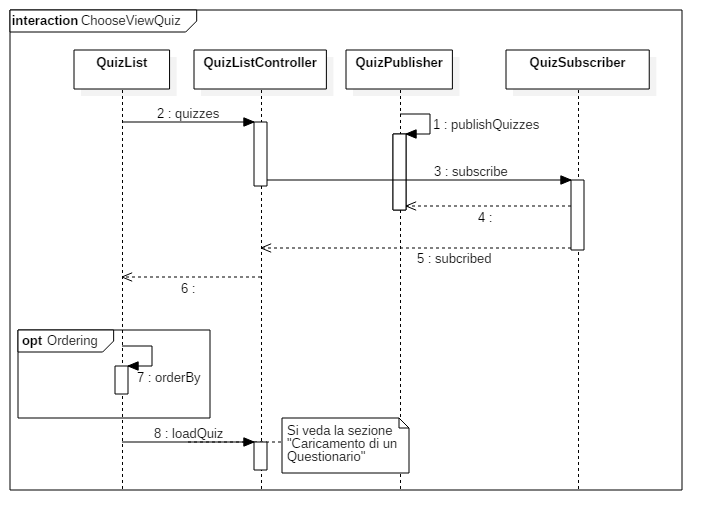
\includegraphics[scale=0.6]{../images/ChooseViewQuiz.png}
		\caption{Diagramma di sequenza sulla visualizzazione e scelta di un questionario}
	\end{center}
	\end{figure}
	\begin{itemize}
	\item\textbf{Precondizioni:} L'utente, intenzionato a svolgere un questionario, accede alla pagina adibita alla selezione dell'argomento.\\
	\item\textbf{Postcondizioni:} L'utente ha scelto un questionario da svolgere e viene reindirizzato alla pagina contenente tale questionario.\\ %è giusta solo questa post o c'è altro?
	\item\textbf{Descrizione:} \textbf{DA CORREGGERE}\textit{La classe CurrentView della View interagisce con la classe InputManager
del Presenter richiedendo un elenco di questionari da visualizzare.} La richiesta viene
inoltrata al Model che procede a recuperare i dati richiesti e a restituirli alla View. Opzionalmente
l’utente ha la possibilità di ordinare i questionari su schermo secondo vari criteri
(alfabetico o cronologico). L’utente ha poi la possibilità di scegliere un questionario e il flusso di eventi si collegherà con quello espresso nel diagramma della sezione "Caricamento
di un Questionario".
	\end{itemize}
	\newpage
	
	\subsection{Caricamento di un Questionario}
	\begin{figure}[h!]
	\begin{center}
		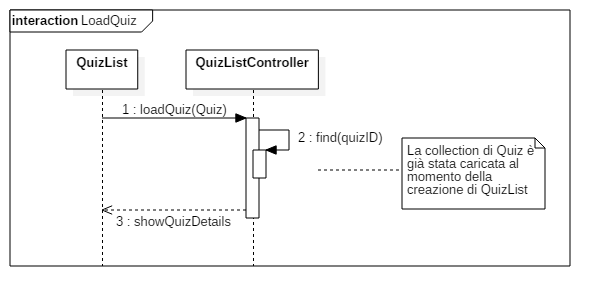
\includegraphics[scale=0.55]{../images/LoadQuiz.png}
		\caption{Diagramma di sequenza sul caricamento di un questionario}
	\end{center}
	\end{figure}
	\begin{itemize}
	\item\textbf{Precondizioni:} L'utente sta entrando in una pagina contenente un questionario che verrà caricato on demand.\\
	\item\textbf{Postcondizioni:} Il questionario è stato correttamente caricato e viene visualizzato a schermo pronto per la risoluzione.\\
	\item\textbf{Descrizione:} L'input iniziale che parte dalla View alla ViewModel contiene l' identificativo del questionario scelto dall'utente. La ViewModel inoltra successivamente questa informazione al Model che si occuperà di estrarre dal database i dati necessari alla costruzione del questionario (effettuata poi dal QuizManager). Una volta assemblato il questionario è pronto per essere somministrato all'utente (il cui diagramma di sequenza è riportato nella sezione "Svolgimento di un Questionario").
	\end{itemize}
	\newpage
	\subsection{Traduzione di una domanda}
	\begin{figure}[h!]
	\begin{center}
		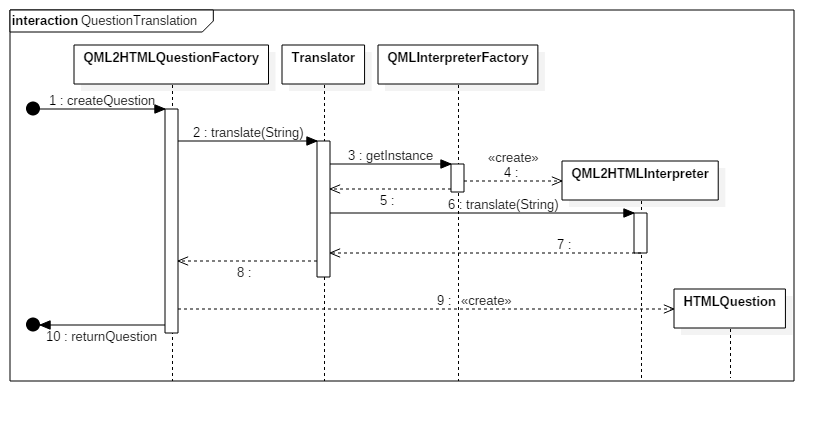
\includegraphics[scale=0.5]{../images/QuestionTranslation.png}
		\caption{Diagramma di sequenza sulla traduzione di una domanda QML}
	\end{center}
	\end{figure}
	\begin{itemize}
	\item\textbf{Precondizioni:} Viene richiesta la visualizzazione su schermo di una domanda.
	\item\textbf{Postcondizioni:} La domanda viene convertita dal precedente formato QML al formato HTML interpretabile dal browser.
	\item\textbf{Descrizione:} alla richiesta di una domanda viene invocata una factory di Question, in questo caso una factory che a partire da testo QML crea domande in HTML. La factory delega la traduzione alla classe Translator; quest'ultima s'interfaccia col package Interpreter, richiedendo l'unica istanza di QMLInterpreterFactory, la quale crea un oggetto QML2HTMLInterpreter. A questo punto Translator può richiedere la traduzione del codice QML all'Interpreter ottenuto, e ritornare il risultato alla QML2HTMLFactory. Infine viene creata la domanda in formato HTML e restituita al richiedente iniziale.
	\end{itemize}
	\newpage
	
	\subsection{Svolgimento di un Questionario}
	\begin{figure}[h!]
	\begin{center}
		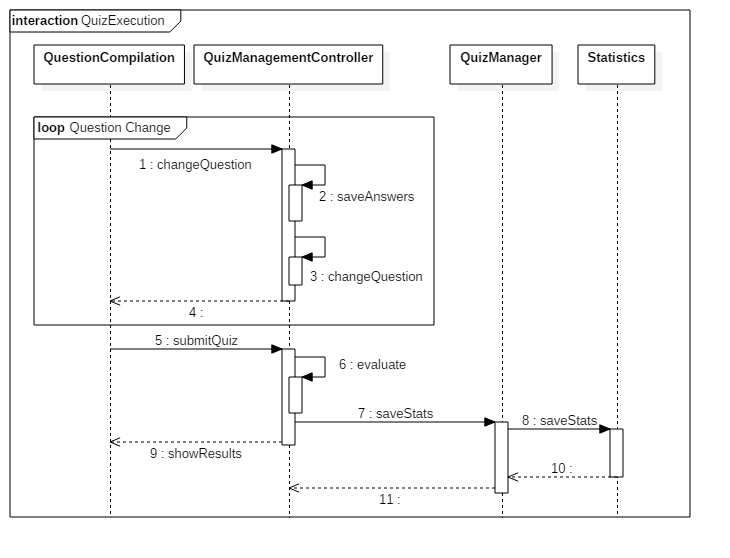
\includegraphics[scale=0.5]{../images/QuizExecution.png}
		\caption{Diagramma di sequenza sullo svolgimento di un questionario}
	\end{center}
	\end{figure}
	\begin{itemize}
	\item\textbf{Precondizioni:} L'utente è intenzionato a svolgere un questionario ed è entrato nella pagina corrispondente a tale questionario. Inizialmente tutte le domande risultano senza risposta. \\
	\item\textbf{Postcondizioni:} L'utente ha svolto il questionario e il sistema, dopo aver compiuto la valutazione, comunica i risultati della prova.\\
	\item\textbf{Descrizione:} Come descritto nel diagramma (evento loop Question Change), l'utente ha la possibilità di scorrere più volte le domande del questionario in modo da risolverle nell'ordine in cui si sente più confortevole. Ogni volta che l'utente richiede la visualizzazione di un'altra domanda il sistema memorizza la risposta fornita dall'utente alla domanda precedente (se questa risposta era effettivamente stata data). Quando un utente ha risposto a tutte le domande può passare alla consegna del questionario, ciò porta al salvataggio delle statistiche della prestazione corrente nella base di dati e al successivo resoconto di valutazione finale che viene esposto all'utente.\\
	\end{itemize}
	\newpage
	\section{Design pattern utilizzati}
		\subsection{Abstract Factory}
	\begin{figure}[h!]
	\begin{center}
		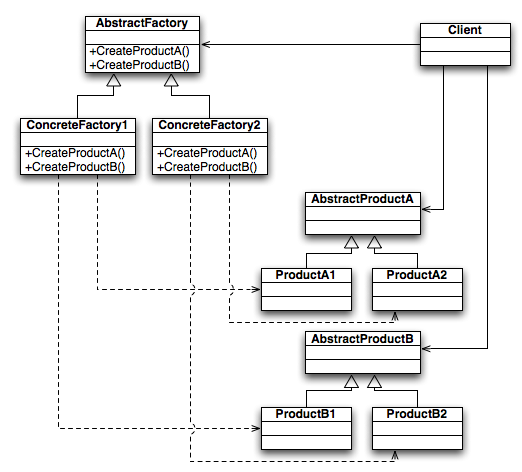
\includegraphics[scale=1]{../images/AbsFactory.png}
		\caption{Design Pattern Abstract Factory}
	\end{center}
	\end{figure}
	\begin{itemize}
		\item\textbf{Scopo}: fornire al Client un'interfaccia per creare famiglie di prodotti, senza dover esplicitare il nome concreto delle classi a cui si riferisce. La factory, quindi, incapsula le responsabilità per la creazione degli oggetti prodotto.
		\item\textbf{Applicabilità}:
		\begin{itemize}
			\item quando si necessita di rendere indipendente un sistema dalla creazione dei suoi componenti, dalla loro rappresentazione e composizione.
			\item quando si necessita la configurazione di un sistema scegliendo tra più tipologie.
			\item quando si devono gestire famiglie di prodotti correlati tra loro e progettati per essere usati insieme.
			\item quando si vuole rivelare solamente l'interfaccia delle classi all'interno di una libreria.
		\end{itemize}
		\item\textbf{Conseguenze}:
		\begin{itemize}
			\item isola le classi concrete, controllandone la creazione. La creazione è delegata
alla classe astratta e i Client manipolano solamente interfacce non conoscendo
i nomi dei prodotti nascosti
			\item permette di modificare facilmente la famiglia di prodotti utilizzati poiché la
classe concreta appare una sola volta nel programma
			\item promuove la coerenza nell'utilizzo dei prodotti poiché sono stati progettati per
essere utilizzati insieme (si usano oggetti di una sola famiglia per volta)
			\item risulta invece difficile l'inserimento di nuove tipologie di prodotto poichè richiederebbe la modifica della classe di Abstract Factory e di conseguentemente il
cambiamento di tutte le sottoclassi (il problema può essere evitato mediante
una tecnica di implementazione della classe astratta, ma in modo meno flessibile e poco sicuro.
		\end{itemize}
		\item\textbf{Utilizzo}: nel sistema Quizzipedia il design pattern è stato utilizzato nei package Interpreter e QuestionManager. Entrambi si avvalgono del pattern per rendere il sistema indipendente dalla creazione delle rispettive classi concrete e rendere i package aperti all'estensione tramite la definizione di nuovi tipi "Interpreter" e "Question".
	\begin{figure}[h!]
	\begin{center}
		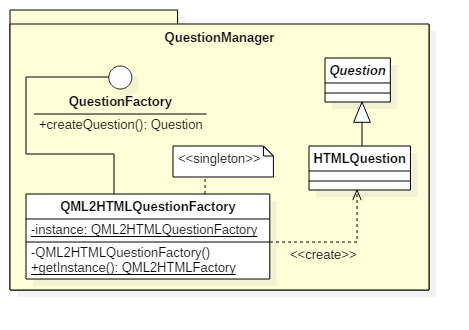
\includegraphics[scale=0.6]{../images/QuestionManagerClassDesignPattern.png}
		\caption{Abstract Factory in QuestionManager}
	\end{center}
	\end{figure}
	\begin{figure}[h!]
	\begin{center}
		\includegraphics[scale=0.5]{../images/interpreterClass.png}
		\caption{Abstract Factory in Interpreter}
	\end{center}
	\end{figure}
	\end{itemize}
	
	\subsection{Singleton}
	\begin{figure}[h!]
	\begin{center}
		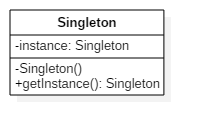
\includegraphics[scale=0.7]{../images/Singleton.png}
		\caption{Design Pattern Singleton}
	\end{center}
	\end{figure}
	\begin{itemize}
		\item\textbf{Scopo}: assicurare l'esistenza di una sola istanza di un oggetto, offrendo un punto globale di accesso a tale istanza.
		\item\textbf{Applicabilità}:
		\begin{itemize}
			\item quando deve essere creata una sola istanza di una classe e deve esistere un punto di accesso ad essa noto a tutti Client
			\item quando l'istanza deve poter essere estesa e i Client devono essere in grado di
utilizzarne le istanze senza apportare modifiche al proprio codice
		\end{itemize}
		\item\textbf{Conseguenze}:
		\begin{itemize}
			\item l'accesso all'unica istanza è controllato
			\item permette di aver un miglior uso delle variabili globali, riducendo lo spazio dei nomi senza inquinarlo con variabili utilizzate per memorizzare riferimenti ad
istanze
			\item maggior  flessibilità per quanto riguarda le operazioni di classe, ma maggior
difficoltà nelle modifiche del progetto per utilizzare più istanze. Impossibilità
di sovrascrivere le funzioni di classe poiché statiche e non virtuali.
		\end{itemize}
		\item\textbf{Utilizzo}: nel sistema Quizzipedia il design pattern è stato utilizzato per le classi\\
		 QML2HTMLQuestionFactory e QMLInterpreterFactory. Usato in collaborazione con\\ l'\emph{Abstract Factory}, il pattern assicura che la costruzione degli oggetti Interpreter e Question abbia un unico punto d'accesso nelle classi sopracitate.
	\end{itemize}
	\newpage
	
	\subsection{Builder}
	\begin{figure}[h!]
	\begin{center}
		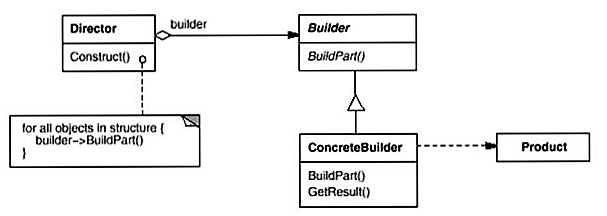
\includegraphics[scale=1]{../images/Builder.png}
		\caption{Design Pattern Builder}
	\end{center}
	\end{figure}
	\begin{itemize}
		\item\textbf{Scopo}: Separa la costruzione di un oggetto complesso dalla sua rappresentazione.
		\item\textbf{Applicabilità}:
		\begin{itemize}
			\item La procedura di creazione di un oggetto complesso
deve essere indipendente dalle parti che
compongono l'oggetto
			\item Il processo di costruzione deve permettere diverse
rappresentazioni per l'oggetto da costruire.
		\end{itemize}
		\item\textbf{Conseguenze}:
		\begin{itemize}
			\item Facilita le modifiche alla rappresentazione interna di
un prodotto
			\item Isola il codice dedicato alla costruzione di un prodotto
dalla sua rappresentazione
			\item Consente un controllo migliore del processo di
costruzione
		\end{itemize}
		\item\textbf{Utilizzo}: nel sistema Quizzipedia il design pattern è stato utilizzato nel package QuizManager per rendere la creazione di un Quiz indipendente dalle domande che lo compongono.
		\begin{figure}[h!]
	\begin{center}
		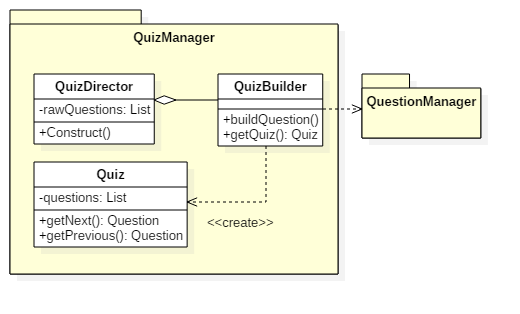
\includegraphics[scale=0.54]{../images/QuizManagerClass.png}
		\caption{Builder in QuizManager}
	\end{center}
	\end{figure}
	\end{itemize}
	\newpage
	
	\subsection{Command}
	\begin{figure}[h!]
	\begin{center}
		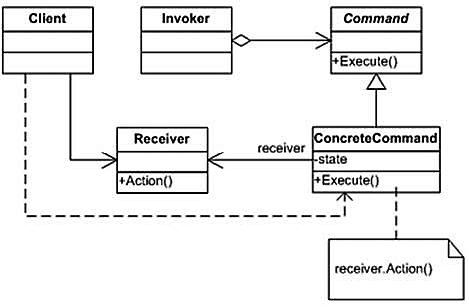
\includegraphics[scale=1]{../images/Command.png}
		\caption{Design Pattern Command}
	\end{center}
	\end{figure}
	\begin{itemize}
		\item\textbf{Scopo}: Incapsulare una richiesta in un oggetto, cosicché i
client sia indipendenti dalle richieste
		\item\textbf{Applicabilità}:
		\begin{itemize}
			\item Necessità di gestire richieste di cui non si conoscono i
particolari
			\item Parametrizzazione di oggetti sull'azione da eseguire
			\item Specificare, accodare ed eseguire richieste molteplici
volte
			\item Supporto ad operazioni di Undo e Redo e a transazioni.
		\end{itemize}
		\item\textbf{Conseguenze}:
		\begin{itemize}
			\item Accoppiamento "lasco" tra oggetto invocante e
quello che porta a termine l'operazione
			\item I command possono essere estesi
			\item I command possono essere composti e innestati
			\item È facile aggiungere nuovi comandi, le classi esistenti non devono essere modificate.
		\end{itemize}
		\item\textbf{Utilizzo}: nel sistema Quizzipedia il design pattern è stato utilizzato nel package Presenter, per disaccoppiare la ricezione degli input da parte della classe InputManager dalla loro risoluzione da parte di altre classi del Presenter e del Model. Il pattern permette inoltre di aggiungere facilmente nuovi \emph{Command} al sistema, estendendo l'interfaccia \emph{Input} del package UserInputManager. Sarà in questo modo più facile estendere le funzionalità offerte all'utente dal sistema Quizzipedia.
	\end{itemize}
	\begin{figure}[h!]
	\begin{center}
		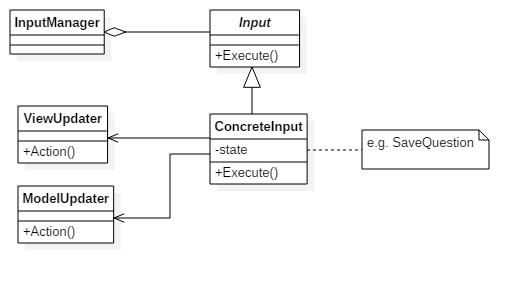
\includegraphics[scale=0.7]{../images/PresenterCommandDesignPattern.png}
		\caption{Design Pattern Command nel Presenter}
	\end{center}
	\end{figure}
	\newpage
	
	\section{Tracciamento}
		\subsection{Mappatura componenti-requisiti}
	\begin{longtable}{p{0.8\textwidth}p{0.20\textwidth}}
\caption{Mappatura dei componenti sui requisiti} \\

Nome componente & Codice requisito \\
\midrule
\endfirsthead

Nome componente & Codice requisito \\
\midrule
\endhead

\multicolumn{2}{c}{\footnotesize\itshape\tablename~\thetable: Mappatura dei componenti sui requisiti}
\endfoot

\multicolumn{2}{c}{\footnotesize\itshape\tablename~\thetable: Mappatura dei componenti sui requisiti}
\endlastfoot

%  M	O	D	E	L

% mancano quelli con scritto ancora non tracciabile

Model::Database 	
							& F 1.2.2\\
							
							& F 2.3.1.1\\
							& F 3\\
							& F 3.1.1\\
							& F 3.2\\
							& F 4\\
							& F 4.5\\
							& F 5\\
							& F 5.2.2\\
							& F 6.2.2\\
\midrule
Model::Database::QuestionManager::AddQuestion	& F 5.2.2.1\\
										
\midrule
Model::Database::QuestionManager::RemoveQuestion	& Non tracciabile\\

\midrule
Model::Database::QuizManager::AddQuiz	& F 6.2.2.1\\

\midrule
Model::Database::QuizManager::RemoveQuiz	& Non tracciabile\\

\midrule
Model::Database::UserManager::LogIn	& Non tracciabile\\

\midrule
Model::Database::UserManager::AddUser	& Non tracciabile\\

\midrule
Model::Database::UserManager::RemoveUser	& Non tracciabile\\

\midrule
Model::Parser::Parser		& F 5.2.1\\

\midrule
Model::Statistics::Statistics	& Non tracciabile\\

\midrule
Model::Publishers::UserPublishers	& Non tracciabile\\

\midrule
Model::Publishers::QuizPublishers	& Non tracciabile\\

\midrule
Model::Publishers::QuestionPublishers	& Non tracciabile\\

%  V	I	E	W   quasi completo 

\midrule
View::Pages::RegistrationPage	& F 1\\
								& F 1.1\\
								& F 1.1.1\\
								& F 1.1.2\\
								& F 1.1.2.1\\
								& F 1.2\\
								& F 1.2.1.1\\
								& F 1.2.1.2\\
								& F 1.2.3\\
\midrule
View::Pages::LoginPage			& F 2\\
								& F 2.1\\
								& F 2.1.1\\
								& F 2.1.2\\
								& F 2.3\\
								& F 2.3.1\\
								& F 2.3.1.1\\
								& F 2.3.2\\
								
\midrule
View::Pages::CategoryListPage					& F 3.1\\
								& F 3.1.1\\
								& F 3.1.2\\
								& F 3.1.3\\

\midrule
View::Pages::QuizListPage					& F 3\\
								& F 3.1\\
								& F 3.1.1\\
								& F 3.1.2\\
								& F 3.1.3\\
								& F 3.2\\
								& F 3.2.1\\
								& F 3.2.2\\
								& F 3.2.3\\
								
\midrule
View::Pages::QuizExecutionPage
								& F 4.1\\
								& F 4.2.1\\
								& F 4.2.2\\
								& F 4.2.3\\
								& F 4.2.4\\
								& F 4.2.4.1\\
								& F 4.2.5\\
								& F 4.2.5.1\\
								& F 4.2.6\\
								& F 4.2.6.1\\
								& F 4.2\\
								& F 4.3\\
								& F 4.4\\
								& F 4.5.1\\
								& F 4.5.2.1\\
								& F 4.5.2.1\\
								& F 4.5.2.1.1\\
								& F 4.5.2.1.2\\
								& F 4.5.2.1.3\\
								& F 4.6.2\\
& F 4.7\\

\midrule
View::Pages::PasswordRecoveryPage	& F 2.2\\
								& F 2.2.1\\
								& F 2.2.2\\
								& F 2.2.2.1\\
								& F 2.2.2.2\\
								& F 2.2.3\\

%mancano questi

\midrule
View::Pages::QuizResultPage	& Non traccibile\\	
							
\midrule
View::Pages::QuizManagementPage	& Non tracciabile\\

\midrule
View::Pages::ViewTutorialPage	& Non tracciabile\\

\midrule
View::Pages::QuizCreationPage	& Non tracciabile\\

\midrule
View::Pages::QuestionCreationPage	& Non tracciabile\\

\midrule
View::Pages::QuestionUpdatePage	& Non tracciabile\\

% templates TO DO

\midrule
View::Templates::QuestionList	& Non tracciabile\\
\midrule
View::Templates::Question	& Non tracciabile\\
\midrule
View::Templates:QuizList:	& Non tracciabile\\
\midrule
View::Templates::Quiz	& Non tracciabile\\
\midrule
View::Templates::QuestionForm	& Non tracciabile\\
\midrule
View::Templates::QuizCreationForm	& Non tracciabile\\
\midrule
View::Templates::QuestionCompilation	& Non tracciabile\\
\midrule
View::Templates::QuizResults	& Non tracciabile\\
\midrule
View::Templates::RegistrationForm	& Non tracciabile\\
\midrule
View::Templates::LoginForm	& Non tracciabile\\
\midrule
View::Templates::PasswordRecoveryForm	& Non tracciabile\\
\midrule
View::Templates::SearchForm	& Non tracciabile\\


%  V	I	E	W	M	O	D	E	L

% package controller TO DO

\midrule
ViewModel::Controllers::NewQuestionController	& Non tracciabile\\
\midrule
ViewModel::Controllers::NewQuizController	& Non tracciabile\\
\midrule
ViewModel::Controllers::QuestionManagementController	& Non tracciabile\\
\midrule
ViewModel::Controllers::DeleteQuestionController	& Non tracciabile\\
\midrule
ViewModel::Controllers::DeleteQuizController	& Non tracciabile\\
\midrule
ViewModel::Controllers::QuizManagementController	& Non tracciabile\\
\midrule
ViewModel::Controllers::QuizListController	& Non tracciabile\\
\midrule
ViewModel::Controllers::QMLEditorController	& Non tracciabile\\
\midrule
ViewModel::Controllers::QuizDetailsController	& Non tracciabile\\

% package subscribers OK

\midrule
ViewModel::Subscribers::QuestionSubscriber	& Non tracciabile\\
\midrule
ViewModel::Subscribers::QuizSubscriber	& Non tracciabile\\
\midrule
ViewModel::Subscribers::UserSubscriber	& Non tracciabile\\

% package methods OK

\midrule
ViewModel::Methods::QuestionMethods	& Non tracciabile\\
\midrule
ViewModel::Methods::QuizMethods	& Non tracciabile\\
\midrule
ViewModel::Methods::UserMethods	& Non tracciabile\\

% package interpreter OK

\midrule
ViewModel::Interpreter::QMLInterpreterFactory	& F 8\\
												
\midrule
ViewModel::Interpreter::QMLInterpreter	& F 8.1\\
										& F 8.2\\
\midrule
ViewModel::Interpreter::QML2HTMLInterpreter	& F 8\\
											& F 8.1\\
											& F 8.2\\
\midrule
							
	\end{longtable}			
	\newpage
		\subsection{Mappatura requisiti - componenti}

\begin{longtable}{p{0.20\textwidth}p{0.80\textwidth}}
\caption{Mappatura dei requisiti sui componenti} \\

Codice Requisito & Nome Componente \\
\midrule
\endfirsthead

Codice Requisito & Nome Componente \\
\midrule
\endhead

\multicolumn{2}{c}{\footnotesize\itshape\tablename~\thetable: Mappatura dei requisiti sui componenti}
\endfoot

\multicolumn{2}{c}{\footnotesize\itshape\tablename~\thetable: Mappatura dei requisiti sui componenti}
\endlastfoot

F 1 & View::CurrentViewManager::CurrentView\\
	& View::UserAuthentication::User\\
\midrule
F 1.1 & View::CurrentViewManager::CurrentView\\
	& View::UserAuthentication::User\\
\midrule
F 1.1.1 & View::CurrentViewManager::CurrentView\\
	& View::UserAuthentication::User\\
\midrule
F 1.1.2 & View::CurrentViewManager::CurrentView\\
	& View::UserAuthentication::User\\
\midrule
F 1.1.2.1 & View::CurrentViewManager::CurrentView\\
	& View::UserAuthentication::User\\
\midrule
F 1.2 & View::CurrentViewManager::CurrentView\\
	& View::UserAuthentication::User\\
\midrule
F 1.2.1 & View::CurrentViewManager::CurrentView\\
	& View::UserAuthentication::User\\
\midrule
F 1.2.1.1 & View::CurrentViewManager::CurrentView\\
	& View::UserAuthentication::User\\
\midrule
F 1.2.1.2 & View::CurrentViewManager::CurrentView\\
			& View::UserAuthentication::User\\
			& Presenter::UserInputManager::Input\\
			& Presenter::UserInputManager::UserRegistration\\
			& Presenter::UserInputManager::InputManager\\
			& Presenter::Updaters::ModelUpdater\\
			& Presenter::Updaters::ViewUpdater\\
			& Model::Database\\
\midrule
F 1.2.1.3 	& View::CurrentViewManager::CurrentView\\
			& View::UserAuthentication::User\\
\midrule
F 1.2.2 & View::CurrentViewManager::CurrentView\\
			& View::UserAuthentication::User\\
			& Presenter::UserInputManager::Input\\
			& Presenter::UserInputManager::UserRegistration\\
			& Presenter::UserInputManager::InputManager\\
			& Presenter::Updaters::ModelUpdater\\
			& Presenter::Updaters::ViewUpdater\\
			& Model::Database\\
\midrule
F 1.2.3 & View::CurrentViewManager::CurrentView\\
			& View::UserAuthentication::User\\
			& Presenter::UserInputManager::Input\\
			& Presenter::UserInputManager::UserRegistration\\
			& Presenter::UserInputManager::Login\\
			& Presenter::UserInputManager::InputManager\\
			& Presenter::Updaters::ModelUpdater\\
			& Presenter::Updaters::ViewUpdater\\
			& Model::Database\\
\midrule
F 2 & View::CurrentViewManager::CurrentView\\
			& View::UserAuthentication::User\\
			& Presenter::UserInputManager::Input\\
			& Presenter::UserInputManager::Login\\
			& Presenter::UserInputManager::InputManager\\
			& Presenter::Updaters::ModelUpdater\\
			& Presenter::Updaters::ViewUpdater\\
			& Model::Database\\
\midrule
F 2.1 	& View::CurrentViewManager::CurrentView\\
			& View::UserAuthentication::User\\
\midrule
F 2.1.1 	& View::CurrentViewManager::CurrentView\\
			& View::UserAuthentication::User\\
\midrule
F 2.1.2 	& View::CurrentViewManager::CurrentView\\
			& View::UserAuthentication::User\\
\midrule



%facoltativi
\iffalse
F 2.2 	& View::CurrentViewManager::CurrentView\\
			& View::UserAuthentication::User\\
\midrule
F 2.2.1 	& View::CurrentViewManager::CurrentView\\
			& View::UserAuthentication::User\\
\midrule
F 2.2.2 	& View::CurrentViewManager::CurrentView\\
			& View::UserAuthentication::User\\
\midrule
F 2 & View::CurrentViewManager::CurrentView\\
			& View::UserAuthentication::User\\
			& Presenter::UserInputManager::Input\\
			& Presenter::UserInputManager::Login\\
			& Presenter::UserInputManager::InputManager\\
			& Presenter::Updaters::ModelUpdater\\
			& Presenter::Updaters::ViewUpdater\\
			& Model::Database\\
\midrule
\fi



F 2.3 & View::CurrentViewManager::CurrentView\\
			& View::UserAuthentication::User\\
\midrule
F 2.3.1 & View::CurrentViewManager::CurrentView\\
		& View::UserAuthentication::User\\
\midrule
F 2.3.1.1 & View::CurrentViewManager::CurrentView\\
			& View::UserAuthentication::User\\
			& Presenter::UserInputManager::Input\\
			& Presenter::UserInputManager::Login\\
			& Presenter::UserInputManager::InputManager\\
			& Presenter::Updaters::ModelUpdater\\
			& Presenter::Updaters::ViewUpdater\\
			& Model::Database\\
\midrule
F 2.3.2 & View::CurrentViewManager::CurrentView\\
			& View::UserAuthentication::User\\
			& Presenter::UserInputManager::Input\\
			& Presenter::UserInputManager::Login\\
			& Presenter::UserInputManager::InputManager\\
			& Presenter::Updaters::ModelUpdater\\
			& Presenter::Updaters::ViewUpdater\\
			& Model::Database\\
\midrule
F 3 & View::CurrentViewManager::CurrentView\\
			& View::Pages::QuizListPage\\
\midrule
F 3.1 & View::CurrentViewManager::CurrentView\\
			& View::Pages::QuizListPage\\
\midrule

%tengo qui per comodità
\iffalse
F 3.1.1 & View::CurrentViewManager::CurrentView\\
		& View::Pages::QuizListPage\\
		& Presenter::UserInputManager::Input\\
			& Presenter::UserInputManager::ViewQuizList\\
			& Presenter::UserInputManager::InputManager\\
			& Presenter::Updaters::ViewUpdater\\
			& Presenter::Updaters::ModelUpdater\\
			& Presenter::QuizManager::QuizDirector\\
			& Presenter::QuizManager::QuizBuilder\\
			& Presenter::QuizManager::Quiz\\
			& Presenter::QuizManager::QuizDirector\\
			& Presenter::QuestionManager::QML2HTMLFactory	 \\
			& Presenter::QuestionManager::HTMLQuestion	 \\
			& Presenter::QuestionManager::Translator		 \\	
			& Presenter::Interpreter::QMLInterpreterFactory	 \\
			& Presenter::Interpreter::QML2HTMLInterpreter		
			& Model::Database\\
\midrule
\fi

F 3.1.1 & View::CurrentViewManager::CurrentView\\
		& View::CurrentViewManager::CurrentView\\
		& View::Pages::QuizListPage\\
		& Presenter::UserInputManager::Input\\
			& Presenter::UserInputManager::ViewQuizList\\
			& Presenter::UserInputManager::InputManager\\
			& Presenter::Updaters::ViewUpdater\\
			& Presenter::Updaters::ModelUpdater\\
			& Model::Database\\
\midrule
F 3.1.2 & View::CurrentViewManager::CurrentView\\
			& View::Pages::QuizListPage\\
\midrule			
F 3.2 & View::CurrentViewManager::CurrentView\\
			& View::Pages::QuizListPage\\			
\midrule						
F 3.2.1 & View::CurrentViewManager::CurrentView\\
		& View::Pages::QuizListPage\\	
		& Presenter::UserInputManager::Input\\
		& Presenter::UserInputManager::ChooseQuiz\\
		& Presenter::UserInputManager::InputManager\\
		& Presenter::Updaters::ModelUpdater\\
		& Presenter::Updaters::ViewUpdater\\
		& Presenter::QuizManager::QuizDirector\\
		& Presenter::QuizManager::QuizBuilder\\
		& Presenter::QuizManager::Quiz\\
		& Presenter::QuizManager::QuizDirector\\
		& Model::Database\\
\midrule
F 3.2 & View::CurrentViewManager::CurrentView\\
		& View::Pages::QuizListPage\\		
\midrule	
F 4		& View::CurrentViewManager::CurrentView\\
		& View::Pages::QuizListPage\\
		& View::Pages::QuizExecutionPage\\
\midrule
F 5		& View::CurrentViewManager::CurrentView\\
		& Presenter::UserInputManager::CreateQuestion\\
		& Presenter::UserInputManager::SaveQuestion	\\
		& Presenter::Updaters::ModelUpdater\\
		& Presenter::QuestionManager::QML2HTMLFactory	 \\
			& Presenter::QuestionManager::HTMLQuestion	 \\
			& Presenter::QuestionManager::Translator		 \\	
			& Presenter::Interpreter::QMLInterpreterFactory	 \\
			& Presenter::Interpreter::QML2HTMLInterpreter\\
			& Model::Database\\
\midrule
F 6		& View::CurrentViewManager::CurrentView\\
& Presenter::UserInputManager::InputManager	\\	
		& Presenter::UserInputManager::CreateQuestion\\
		& Presenter::UserInputManager::SaveQuestion	\\
		& Presenter::Updaters::ModelUpdater\\
		& Presenter::QuestionManager::QML2HTMLFactory	 \\
			& Presenter::QuestionManager::HTMLQuestion	 \\
			& Presenter::QuestionManager::Translator		 \\	
			& Presenter::Interpreter::QMLInterpreterFactory	 \\
			& Presenter::Interpreter::QML2HTMLInterpreter\\
			& Presenter::QuizManager::QuizDirector\\
		& Presenter::QuizManager::QuizBuilder\\
		& Presenter::QuizManager::Quiz\\
		& Presenter::QuizManager::QuizDirector\\
		& Model::Database\\
\midrule
F 7 & Presenter::UserInputManager::InputManager	\\	
& View::CurrentViewManager::CurrentView\\
& View::UserAthentication::User\\
& Presenter::UserInputManager::Logout	\\	
& Presenter::Updaters::ViewUpdater\\
& Model::Database\\
			
	\end{longtable}

	
\end{document}
